\documentclass[ xcolor = pdftex, dvipsnames, table ]{beamer}

\usetheme[compress]{Berlin}
\usecolortheme{whale}
\setlength{\parskip}{0.1in}
\usepackage{bm}
\usepackage{tikz}
\usepackage{dsfont}
\usepackage{graphicx}
\usepackage{changepage}
\usepackage{pgfgantt}
\usepackage{nicefrac}
\usepackage{scalerel}
\usepackage{xcolor}
\usepackage[symbol]{footmisc}
%\usepackage{enumitem}


%\title{Baysian Nonparametric Estimation of ODEs as Applied to the Stock Recruitment Relationship}
%\title{Metamodeling for Bias Estimation of Biological Reference Points Under Two-Parameter SRRs}
\title{A Metamodeling Approach for Bias Estimation of Biological Reference Points}
\author{
Nick Grunloh
%\\$~$\\
%In collaboration with:\\
%Dr. E.J. Dick\\
%Dr. H. K.H. Lee
}
\date{13 August 2024}

%
\DeclareMathOperator*{\argmin}{\arg\!\min}
\DeclareMathOperator*{\argmax}{\arg\!\max}

%
\newcommand{\kr}{ \frac{\kappa w_\infty}{w(a_s)} }
\newcommand{\one}{
        \left(\frac{Z(Z+\kappa)}{\alpha w(a_s)(Z+\kr)}\right)^\gamma
}
\newcommand{\two}{
        \left(\frac{\gamma F}{\alpha w(a_s)}\right) \left(\frac{Z(Z+\kappa)}{\alpha w(a_s)(Z+\kr)}\right)^{\gamma-1}
}
\newcommand{\thr}{
        \frac{\left(\kr\right)\left(\kappa-\kr\right)}{(Z+\kr)^2}
}
%
\newcommand{\oneA}{
        \left(\frac{Z^*(Z^*+\kappa)}{w(a_s)(Z^*+\kr)}\right)^\gamma
}
\newcommand{\twoA}{
        \left(\frac{\gamma F^*}{w(a_s)}\right) \left(\frac{Z^*(Z^*+\kappa)}{w(a_s)(Z^*+\kr)}\right)^{\gamma-1}
}
\newcommand{\thrA}{
        \frac{\left(\kr\right)\left(\kappa-\kr\right)}{(Z^*+\kr)^2}
}

%\newenvironment{changemargin}[2]{%
%\begin{list}{}{%
%\setlength{\topsep}{0pt}%
%\setlength{\leftmargin}{#1}%
%\setlength{\rightmargin}{#2}%
%\setlength{\listparindent}{\parindent}%
%\setlength{\itemindent}{\parindent}%
%\setlength{\parsep}{\parskip}%
%}%
%\item[]}{\end{list}}

%\AtBeginSection[]
%{
%    \begin{frame}
%        \frametitle{Table of Contents}
%        \tableofcontents[currentsection, currentsubsection]
%    \end{frame}
%}
%
%\AtBeginSubsection[]
%{
%    \begin{frame}
%        \frametitle{Table of Contents}
%        \tableofcontents[currentsection, currentsubsection]
%    \end{frame}
%}

%
\begin{document}

%
\begin{frame}
\titlepage
\vspace*{-3cm}
\begin{minipage}[h!]{0.49\textwidth}
\hspace*{-0.25cm}

\includegraphics[width=0.6\textwidth]{noaaText.png}
\end{minipage}
\begin{minipage}[h!]{0.49\textwidth}
\hspace*{2cm}

\includegraphics[width=0.55\textwidth]{slug.jpg}
\end{minipage}
\end{frame}

%%
%\begin{frame}{Outline}
%    \tableofcontents
%\end{frame}

%
\section{Introduction}
\subsection{}
\begin{frame}{Outline}
    \tableofcontents[currentsection, currentsubsection]
\end{frame}

%
\begin{frame}
	$~$\\
	\centering
	\begin{tikzpicture}[overlay]
	\node at (0,0) {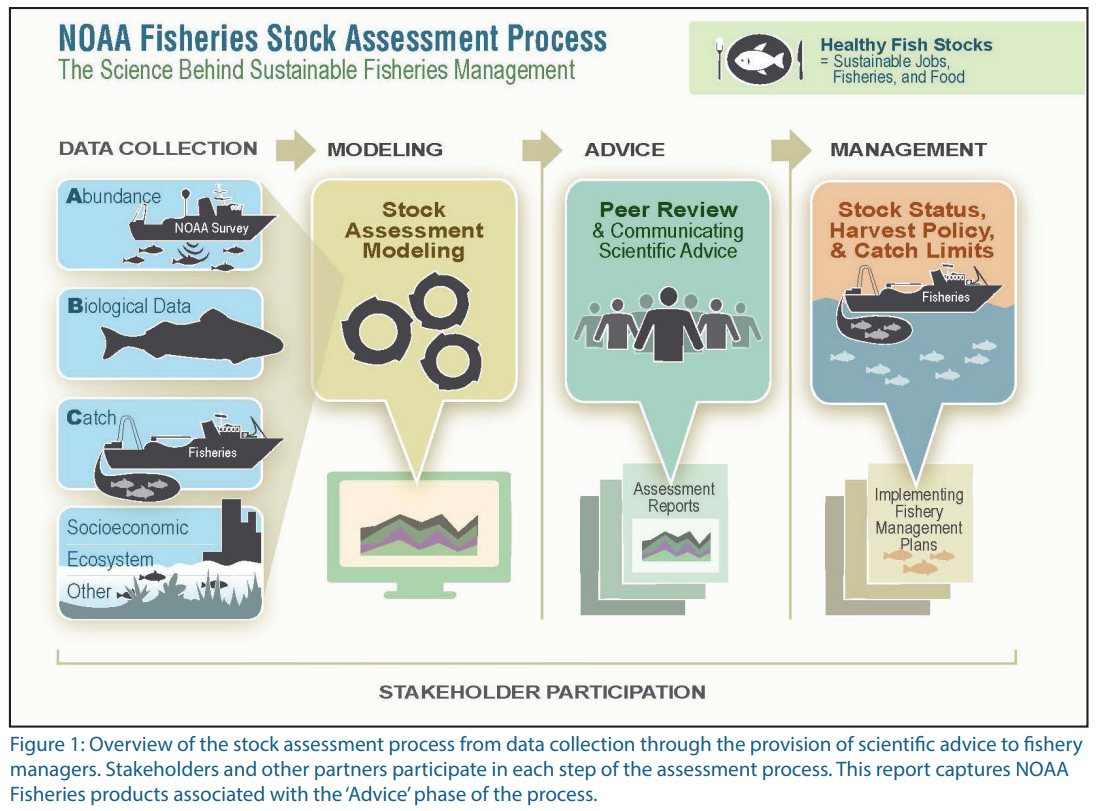
\includegraphics[width=0.8\textwidth]{saCycle.png}\footnote{NOAA Fisheries Annual Stock Assessment Report 2020}};
	\node (a) at (-0.25,-1.65) {};
	\node (b) at (2.5,-1.65) {};
	\onslide<2->{
	\draw[->, line width=1mm] (a) edge[bend right] node[below, near end, text=black]{RPs} (b);
	}
	\end{tikzpicture}
	%*NOAA Fisheries Annual Stock Assessment Report 2020
\end{frame}



%
\begin{frame}{Surplus Production Model General Structure}
	\centering 
	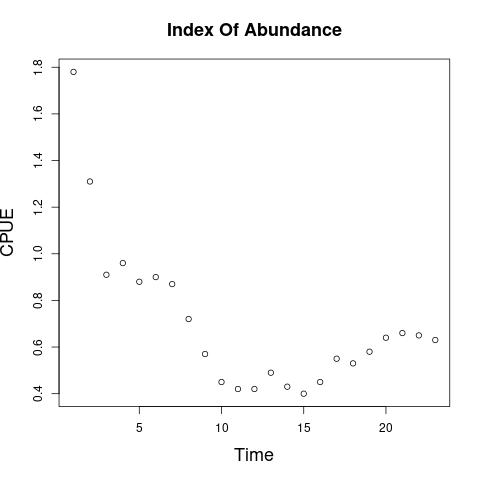
\includegraphics[width=0.4\textwidth]{../plots/hakeIndex.png}
	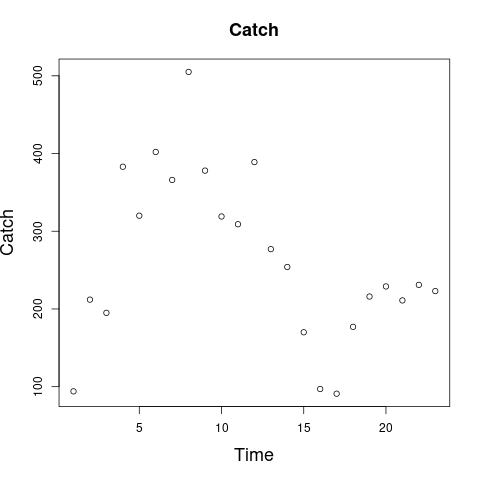
\includegraphics[width=0.4\textwidth]{../plots/hakeCatch.png}
	%
        \begin{align*}
	I_t = q B_t e^\epsilon ~~~ \epsilon\sim N(0, \sigma^2) \label{resp}\\
	~\\
	\frac{dB}{dt} = P(B(t); \bm{\theta}) - Z(t)B(t)
	\end{align*}
	
	%%
	%\begin{equation*}
	%\frac{dB}{dt} = P(B(t); \bm{\theta}) - Z(t)B(t) \label{ode}
	%\end{equation*}
\end{frame}

%
\begin{frame}
\begin{minipage}[h!]{0.49\textwidth}
	Reference Points:
	\begin{itemize}
	\setlength{\itemsep}{5mm}
	\item Maximum Sustainable Yield ($MSY$)
	\item $F_{MSY}$ (or {\tiny$\frac{F_{MSY}}{M}$}): Fishing rate to achieve $MSY$
	\item $\frac{B_{MSY}}{B_0}$: Biomass Depletion when at $MSY$
	\item Driven by the shape of $P$ as determined by $\theta$.
	\end{itemize}
\end{minipage}
\begin{minipage}[h!]{0.49\textwidth}
	\hspace{0.5cm}
	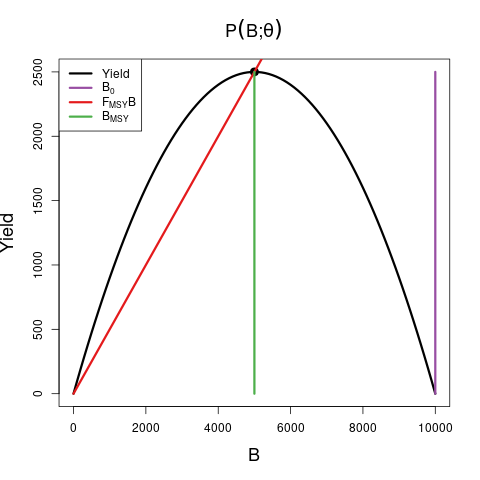
\includegraphics[width=\textwidth]{../../advance/plots/yieldRPplusP.png}
\end{minipage}
\end{frame}

%NOTE: STEP THRU CONSTRAINTS
\begin{frame}
\onslide<1->{
\begin{minipage}[h!]{0.59\textwidth}
Conceptually:
\begin{align*}
\frac{F_{MSY}}{M}\in\mathbb{R}^+ ~~~ \frac{B_{MSY}}{B_{0}}\in\left(0, 1\right)
\end{align*}
}
%$~$\\
%Mangel et al. 2013, CJFAS:
\vspace{-0.5cm}
\begin{itemize}
	\setlength{\itemsep}{5mm}
	\onslide<2->{ \item Schaefer Model: $~ F_{MSY}\in\mathbb{R}^+ ~~~ \frac{B_{MSY}}{\bar B(0)}=\frac{1}{2}$ }
        \onslide<3->{ \item BH Model: $~ \frac{F_{MSY}}{M}\in\mathbb{R}^+ ~~~ \frac{B_{MSY}}{\bar B(0)}=\frac{1}{F_{MSY}/M+2}$ }
        \onslide<4->{
	\item Similar Constraints for other Two-Parameter Models: \\$~~~~~$Fox, Ricker, etc... 
        \item Three-Parameter Models Allow Independent RP Estimation %More flexible models allow independent RP estimation
	}
\end{itemize}
\end{minipage}
\begin{minipage}[h!]{0.39\textwidth}
%$~$\\
\only<1>{ 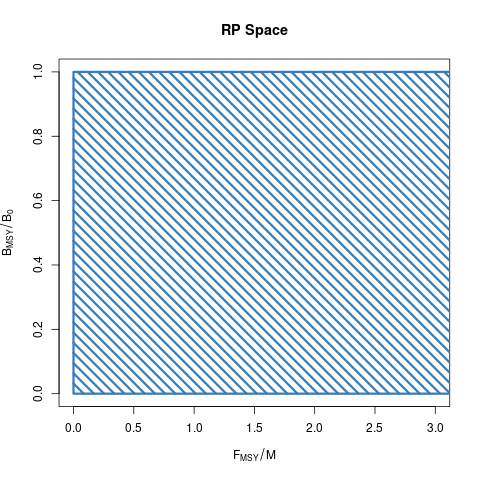
\includegraphics[width=1.2\textwidth]{hatchRP.png} \\$~$\\}
\only<2>{ 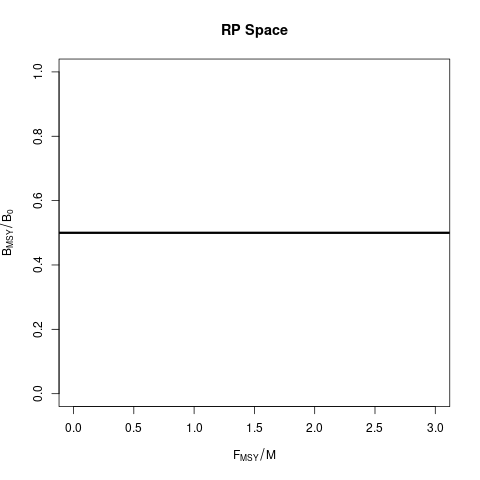
\includegraphics[width=1.2\textwidth]{sRP.png} \\$~$\\}
\only<3>{ 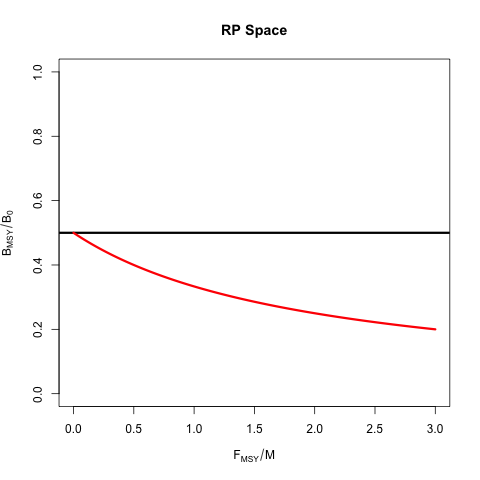
\includegraphics[width=1.2\textwidth]{sbhRP.png} \\$~$\\}
\only<4>{ 
	%$~$\\
	%\hspace*{-0.5cm}
	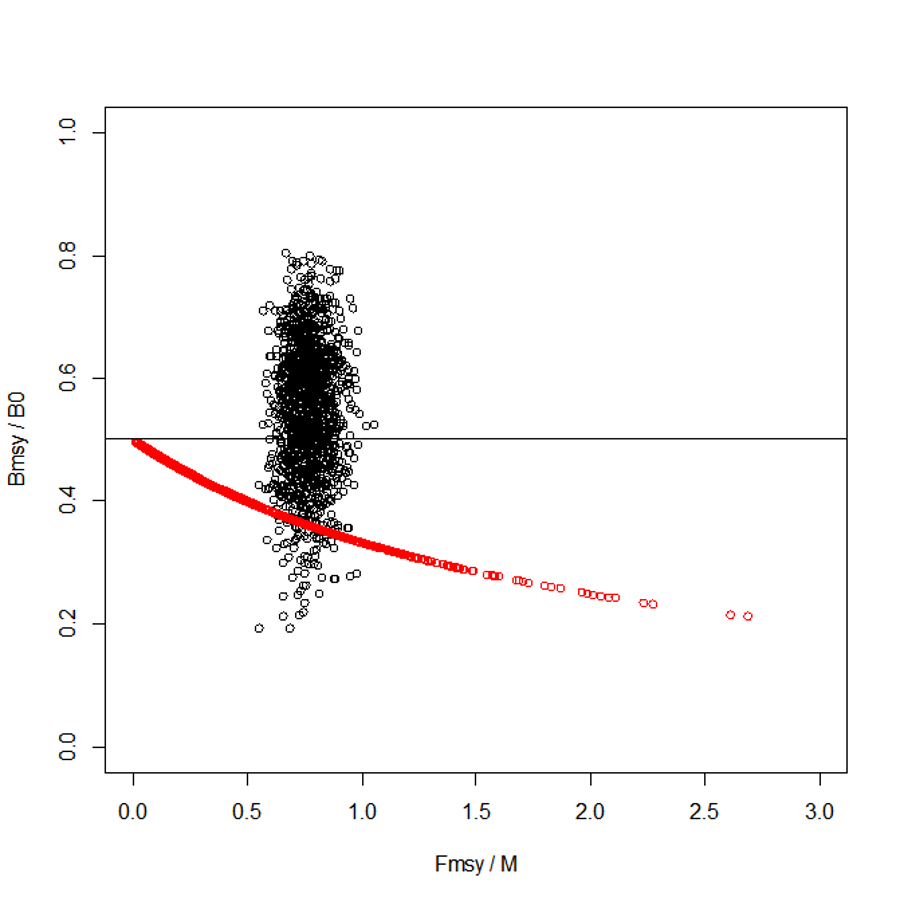
\includegraphics[width=1.2\textwidth]{cjasFig.png}\footnote{\scriptsize Mangel et al. 2013, CJFAS} 
}
\end{minipage}
\end{frame}

%
\begin{frame}

%
\hspace{-1cm}
\begin{minipage}[h!]{0.69\textwidth}
%$~$\\\hspace{-2cm}
\begin{itemize}
%[leftmargin=-2em]
%[align=right,itemindent=2em,labelsep=2pt,labelwidth=1em,leftmargin=0pt,nosep] 
%[leftmargin=*]
%\setlength{\itemindent}{-2em}
%\itemindent=-13pt
%\setlist[itemize]{labelindent=0pt,labelwidth=0pt, labelsep*=0pt, leftmargin=!, style=standard}
\setlength{\itemsep}{5mm}
%\begin{enumerate}[leftmargin=-1pt]
%[align=right,itemindent=2em,labelsep=2pt,labelwidth=1em,leftmargin=0pt,nosep]
%\itemindent=-13pt
\onslide<1->{ 
\item {Two-Parameter models remain standard and can induce biased RP estimation.} %via RP bias.
}
\onslide<2->{
\item Metamodeling RP estimation makes these RP trade-offs explicit. %trade-offs between RPs explicit.
\item Clear description of the induced risk profile of over/under fishing. %clear. %induced by two-parameter RP estimation clear.
%Outlines clear risk profile induced by two-parameter RP estimation.
%\item Inform the utility of SRR flexibility for modelers, managers, and stakeholders.

}
\onslide<3->{
\item Suggests mechanisms and the types of stocks where RP estimation may fail. % as well as mechanisms of failure.
%\item Demonstrate the types of stocks where RP estimation may fail.
%\item Suggest mechanisms for understanding what causes bias. utility of SRR flexibility
\item Demonstrates the utility of adopting more flexible SRR models.
}
%\end{enumerate}
\end{itemize}

%\item 
%By modeling how two-parameter models bias RP estimation, a metamodel of RP estimation  makes trade-offs between RPs explicit, and demonstrates risk profilo of induced by two-parameter models. 
%about trade-offs between RPs so as to 
%\item inform the full utility of reducing bias through more flexible SRRs

%%
%By simulating from three-parameter models and observing RP estimation under misspecified two parameter 
%models, a metamodel of the RP estimation process makes the consquences of RP estimation explicit.
%%
%The metamodel demonstrates the types of stocks where RP estimation may fail, indicates how RP estimation 
%fails, and quantifies the scale of biases. % with current models.
%
%%
%The metamodel is explicit about trade-offs between RPs so as to inform the full utility of reducing bias, 
%as well as to suggest mechanism for understanding what causes bias.
\end{minipage}
\begin{minipage}[h!]{0.38\textwidth}
	%$~$\\
        \begin{tikzpicture}[overlay]
        \node at (2.35,0.4) {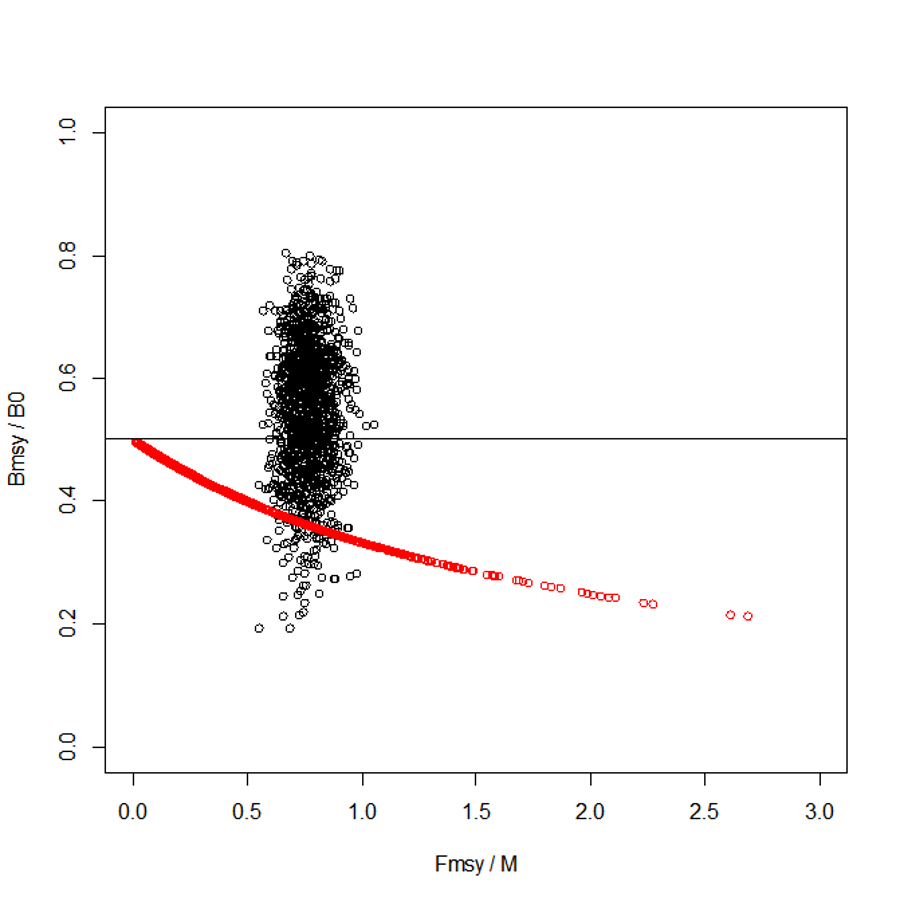
\includegraphics[width=1.25\textwidth]{cjasFig.png}}; %{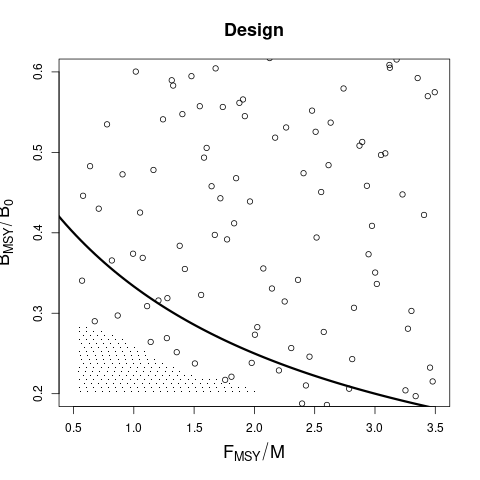
\includegraphics[height=0.7\textheight]{../../gpBias/designLineHHardExpT45N150M0.3Wide.png}};
        \node[circle, fill=white, draw, minimum size=7, inner sep=-2] at (1.55,0.75){\tiny 3}; 
        \node[circle,fill=red, minimum size=7, inner sep=-2] at (1.0,0.2){\tiny 2};
	\draw[latex-, very thick,black] (1.05,0.25) -- ++(0.4,0.45);
        \end{tikzpicture}
%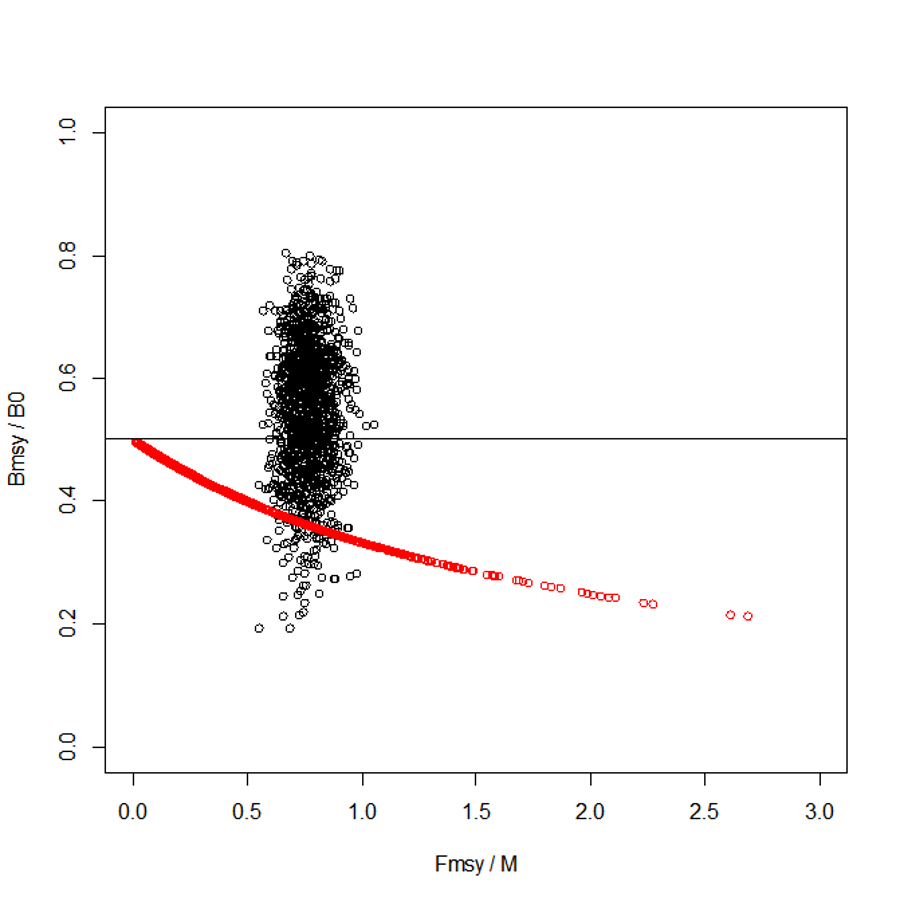
\includegraphics[width=1.2\textwidth]{cjasFig.png}%\footnote{\scriptsize Mangel et al. 2013, CJFAS}
\end{minipage}
\end{frame}


%%
%\begin{frame}
%	%
%	\begin{itemize}
%		\item MSA?
%		\item RPs
%		\item Steepness paper
%	\end{itemize}
%\end{frame}

%
\section{The Schaefer Model}
\subsection{}
\begin{frame}{Outline}
    \tableofcontents[currentsection, currentsubsection]
\end{frame}

%
\begin{frame}
	\begin{minipage}[h!]{0.59\textwidth}
	\begin{itemize}
	\setlength\itemsep{1em}
	\item $P_\ell$ is logistic production
	\item Logistic map in discrete time 
	%\begin{itemize}
	%	\item Quadratic in $B$
	%	\item Discrete time gives the logistic map.
	%\end{itemize}
	\item Implicit Natural Mortality
	\item Explicit Fishing Mortality 
	\end{itemize}
	\end{minipage}
	\begin{minipage}[h!]{0.39\textwidth}
        %
        \begin{align*}
        I_t = q B_t e^\epsilon ~~~ \epsilon\sim N(0, \sigma^2)
        \end{align*}

        %
        \begin{equation*}
        \frac{dB}{dt} = P_\ell(B(t); \bm{\theta}) - F(t)B(t)
        \end{equation*}
	\end{minipage}
%\begin{itemize}
%\color{red}
%\item Observation model
%\item introduce logistic P
%\item something else?
%\end{itemize}
\end{frame}

%
\begin{frame}
%
\begin{minipage}[h!]{0.54\textwidth}
\only<1>{
\begingroup
\scriptsize
\begin{align*}
P_{\ell}(B; [r, K]) &= r B\left(1-\left(\frac{B}{K}\right)\right)\\
\end{align*}
\endgroup
\underline{Reference Points:}
\begin{align*}
F^* &= \frac{r}{2}\\
&\\
B^* = \frac{K}{2} ~~&~~ B_0 = K\\
\frac{B^*}{B_0} &= \frac{1}{2}
\end{align*}
}
\only<2>{
$~$\\
\begingroup
\scriptsize
\begin{align*}
P_{pt}(B; [r, K, \gamma]) &= \frac{r B}{\gamma-1} \left(1-\left(\frac{B}{K}\right)^{(\gamma-1)}\right)
\end{align*}
\endgroup
$~$\\
\underline{Reference Points:}
\begin{align*}
F^* =& \frac{r}{\gamma}~~\\
&\\
B^* = K\left(\frac{1}{\gamma}\right)^{\frac{1}{\gamma-1}} &~~ B_0 = K\\
\frac{B^*}{B_0} =& \left(\frac{1}{\gamma}\right)^{\frac{1}{\gamma-1}}~~
\end{align*}
}
\end{minipage}
\begin{minipage}[h!]{0.44\textwidth}
\only<1>{$~$\\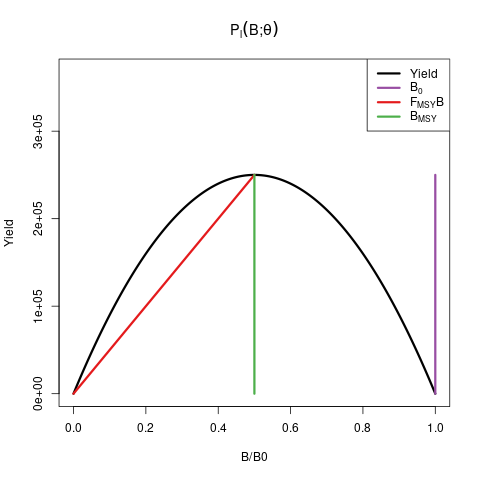
\includegraphics[width=1.1\textwidth]{../../ptNew/g5S.png}}%../plots/srrSchaeffer.png}}
\only<2>{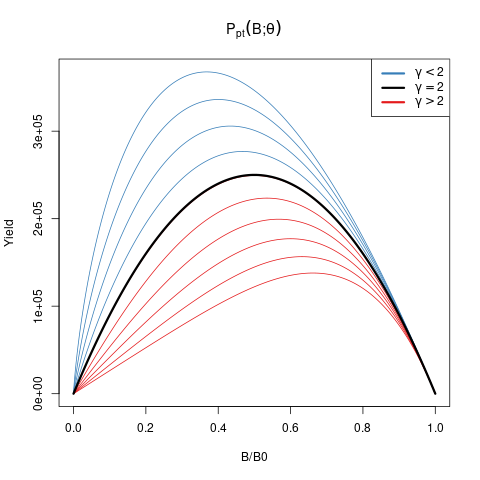
\includegraphics[width=1.1\textwidth]{../../ptNew/g5PT.png}}
\end{minipage}
\end{frame}

%%
%%\begin{frame}
%\begin{align}
%P_{p}(B; [r, K, \gamma]) = \frac{r B}{\gamma-1} \left(1-\left(\frac{B}{K}\right)^{(\gamma-1)}\right). \label{pt}
%\end{align}
%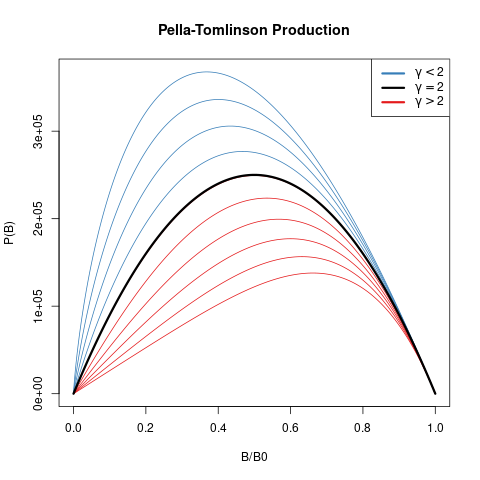
\includegraphics[width=0.49\textwidth]{../../ptNew/g4PT.png}
%\end{frame}

%%
%\begin{frame}
%%
%\begin{equation}
%\frac{dB}{dt} = \frac{r B}{\gamma-1} \left(1-\left(\frac{B}{K}\right)^{\gamma-1}\right) - FB. \label{dBdtPT}
%\end{equation}
%
%%
%\begin{align}
%\bar B(F) = K\left(1-\frac{F(\gamma-1)}{r}\right)^{\frac{1}{(\gamma-1)}}. \label{BbarPT}
%\end{align}
%
%%
%\begin{align}\label{ptRP}
%&F^* = \frac{r}{\gamma}
%&\frac{B^*}{\bar B(0)} = \left(\frac{1}{\gamma}\right)^{\frac{1}{\gamma-1}}
%\end{align}
%
%\end{frame}

%
\begin{frame}
%
\begin{minipage}[h!]{0.59\textwidth}
\only<1>{
%
\begin{align*}\label{ptRP}
&F^* = \frac{r}{\gamma}
&\frac{B^*}{\bar B(0)} = \left(\frac{1}{\gamma}\right)^{\frac{1}{\gamma-1}}
\end{align*}

%
\begin{center}
\begin{tikzpicture}[overlay]
\node at (-2,-0.5) {
\includegraphics[height=0.12\textheight, angle=90]{doubleArrow.png}};
%\vspace*{-2cm}
\node at (0,-0.5) {Closed-Form Inversion};
%\vspace*{-1cm}
\node at (2,-0.5) {
\includegraphics[height=0.12\textheight, angle=270]{doubleArrow.png}};
\end{tikzpicture}
\end{center}

%
$~$\\
\begin{align*}
&r = \gamma F^*
&\gamma = \frac{W\left(\frac{B^*}{\bar B(0)}\log\left(\frac{B^*}{\bar B(0)}\right)\right)}{\log\left(\frac{B^*}{\bar B(0)}\right)}
\end{align*}
}
%\only<2>{
%%
%\begin{align*}\label{ptRP}
%&F^* = \frac{r}{\gamma}
%&\frac{B^*}{\bar B(0)} = \left(\frac{1}{\gamma}\right)^{\frac{1}{\gamma-1}}
%\end{align*}
%
%%
%\begin{center}
%\begin{tikzpicture}[overlay]
%\node at (-2,-0.5) {
\includegraphics[height=0.12\textheight, angle=90]{doubleArrow.png}};
%%\vspace*{-2cm}
%\node at (0,-0.5) {Closed-Form Inversion};
%%\vspace*{-1cm}
%\node at (2,-0.5) {
\includegraphics[height=0.12\textheight, angle=270]{doubleArrow.png}};
%\end{tikzpicture}
%\end{center}
%
%%
%$~$\\
%\begin{align*}
%&r = \gamma F^*
%&\gamma = \frac{W\left(\frac{B^*}{\bar B(0)}\log\left(\frac{B^*}{\bar B(0)}\right)\right)}{\log\left(\frac{B^*}{\bar B(0)}\right)}
%\end{align*}
%}
\only<2>{
%\hspace{-1cm}
\begin{equation*}
\underbrace{\left(F_{MSY}, \frac{B_{MSY}}{\bar B(0)}\right)}_{\text{PT Truth}} {\text{GP}\atop{\mapsto\atop~}} \underbrace{\left(\hat F_{MSY}, \frac{1}{2}\right)}_{\text{Schaefer Estimate}}
\end{equation*}
}
\end{minipage}
\begin{minipage}[h!]{0.39\textwidth}
\begin{center}
\begin{tikzpicture}[overlay]
%\only<1>{
%\node at (0.5,0) {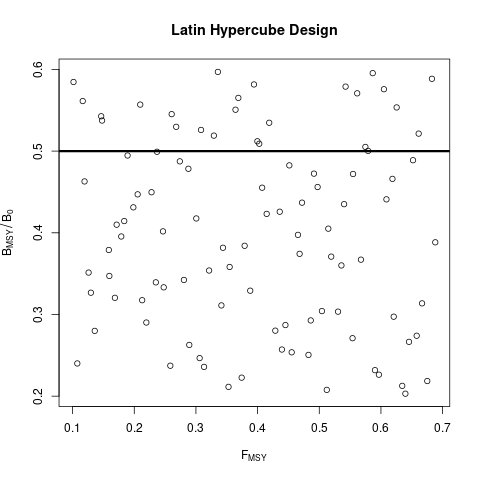
\includegraphics[height=0.65\textheight]{../../ptNew/simplePTDesign.png}};%gpBias/designLineHHardExpT45N150M0.3Wide.png}};
%}
%\only<2>{
\only<1>{
\node at (0.5,-0.2) {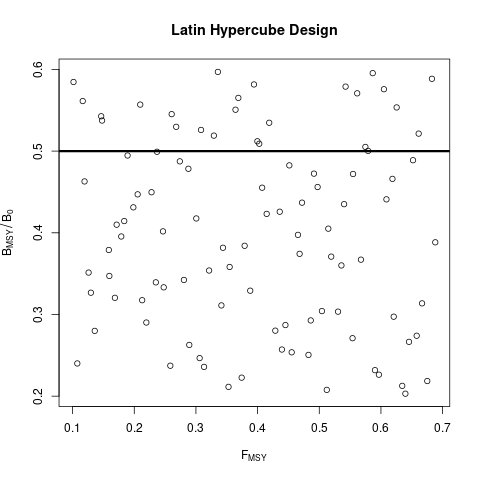
\includegraphics[height=0.65\textheight]{../../ptNew/simplePTDesign.png}};
\node[circle, draw, minimum size=9, inner sep=-2] at (0.6,-1.2){\tiny PT};
\draw[latex-, very thick,black] (0.6,0.65) -- ++ (0,-1.65); %(0.6,-0.9) -- ++(1.9,2.3);
\node[circle,fill=red, minimum size=9, inner sep=-2] at (0.6,0.75){\tiny $\ell$};
}
%\only<3>{
\only<2>{
\node at (0.5,-0.1) {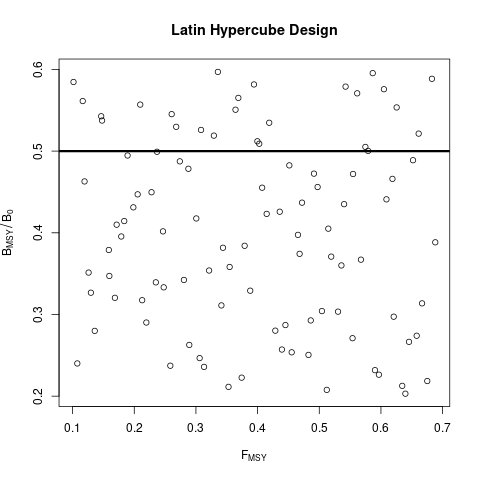
\includegraphics[height=0.65\textheight]{../../ptNew/simplePTDesign.png}};
\node[circle, draw, minimum size=9, inner sep=-2] at (0.6,-1.1){\tiny PT};
\draw[latex-, very thick,black] (0.6,0.75) -- ++ (0,-1.65); %(0.6,-0.9) -- ++(1.9,2.3);
\node[circle,fill=red, minimum size=9, inner sep=-2] at (0.6,0.85){\tiny $\ell$};
}
\end{tikzpicture}
\end{center}

\end{minipage}

%\vspace*{0.5cm}
\only<1>{
$~$

* Lambert $W$ function inverts $xe^x$ $s.t.$ $W(xe^x)=x$
}

%\only<2>{
%$~$
%
%* Lambert $W$ function inverts $xe^x$ $s.t.$ $W(xe^x)=x$
%}
\end{frame}

%%
%\begin{frame}
%\color{red}
%Show GP
%\end{frame}

%
\begin{frame}
%
\begin{minipage}[h!]{0.54\textwidth}
\only<1>{
\begin{align*}
\frac{dB}{dt} &= P(B(t); \theta) - F(t)B(t)\\
	&= P(B(t); \theta) - F^*_\theta\underbrace{\frac{F(t)}{F^*_\theta}}_{\substack{\text{Relative}\\\text{Fishing}}}B(t)\\
\end{align*}
}
\only<2>{
\begin{align*}
&~\\
\frac{dB}{dt} &= P(B(t); \theta) - F(t)B(t)\\
	&= P(B(t); \theta) - \underbrace{F^*_\theta\frac{F(t)}{F^*_\theta}B(t)}_{{\color{red}C(t)}}\\
&~\\
\end{align*}
}
\end{minipage}
\begin{minipage}[h!]{0.34\textwidth}
\only<1>{ 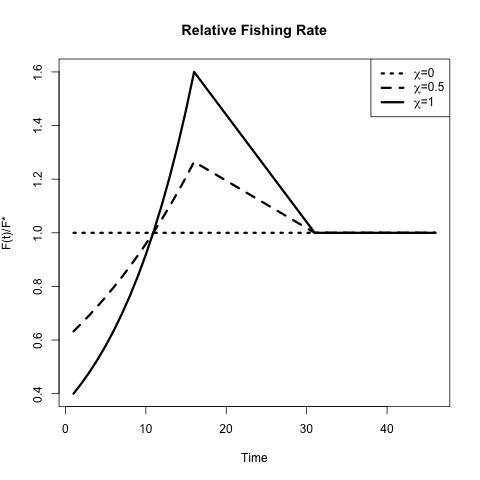
\includegraphics[width=1.5\textwidth]{../../ptNew/relFish.png} }
\only<2>{ 
\begin{tikzpicture}[overlay]
        \node at (2.8,0) {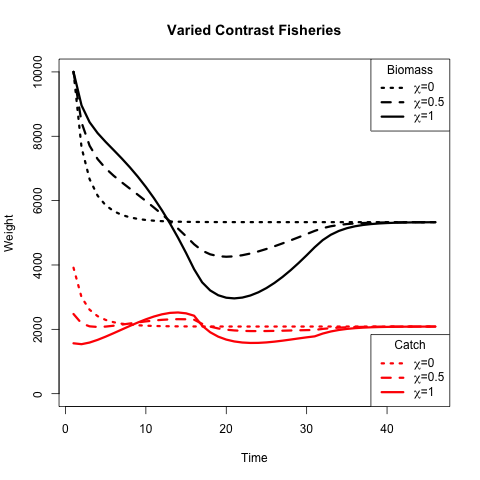
\includegraphics[width=1.5\textwidth]{../../ptNew/relSeries.png}};
	\node at (3,1) {$B(t)$};
	\node at (3,-1.5) {\color{red}$C(t)$};
\end{tikzpicture}
}
\end{minipage}

%%
%\begin{figure}[h!]
%\centering
%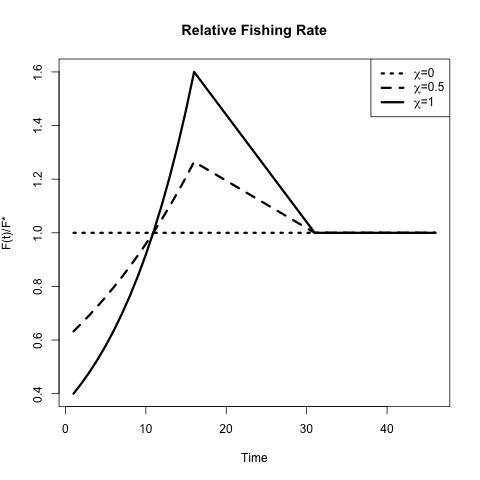
\includegraphics[width=0.44\textwidth]{../../ptNew/relFish.png}
%$~$
%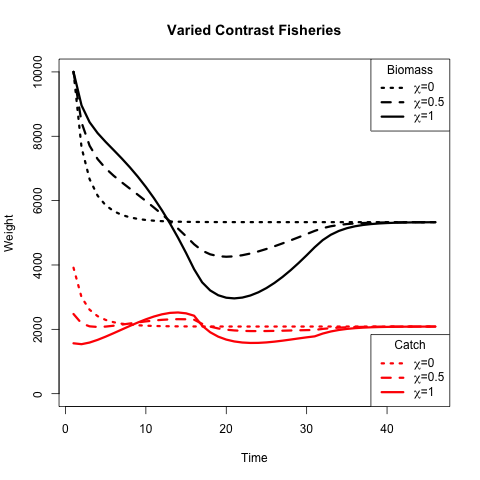
\includegraphics[width=0.44\textwidth]{../../ptNew/relSeries.png}
%%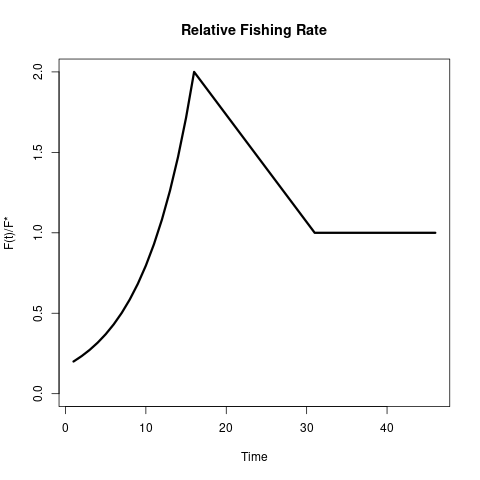
\includegraphics[width=0.45\textwidth]{../../../theses/nick/gpBias/rfExpT45X2Z0.6.png}
%%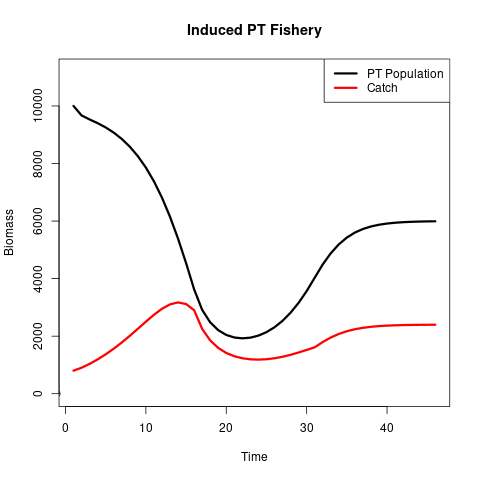
\includegraphics[width=0.45\textwidth]{../../../theses/nick/gpBias/bioCatchExpT45X2Z0.6.png}
%%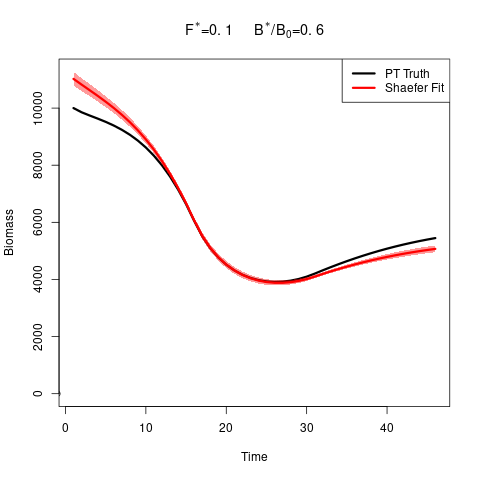
\includegraphics[width=0.5\textwidth]{../../../theses/nick/gpBias/bioPostCompareExpT45X0.5Z0.6.png}
%%\vspace{-1cm}
%\caption{ \label{catchT45}
%($left$) Relative fishing with low, medium, and high contrast.
%($right$) Population biomass and catch at each associated level of contrast. %demonstrating contrast in a {\color{red}PT population} with $F^*=0.4$ and $
%}
%\label{catch45}
%\end{figure}
\end{frame}

%
\begin{frame}
%\begin{figure}[h!]
\begin{minipage}[h!]{0.44\textwidth}
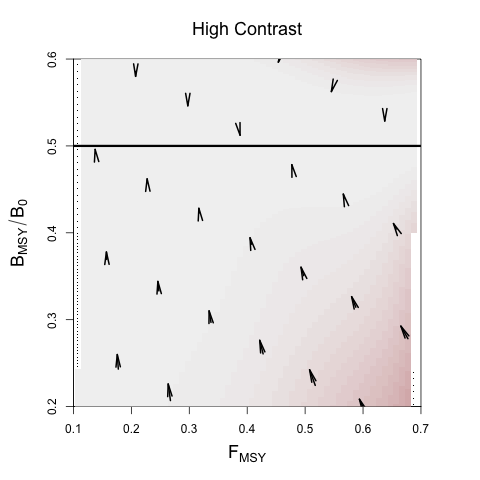
\includegraphics[width=1.1\textwidth]{../../ptNew/directionalBiasSubPTExpT45MinCon.png}
\end{minipage}
\begin{minipage}[h!]{0.44\textwidth}
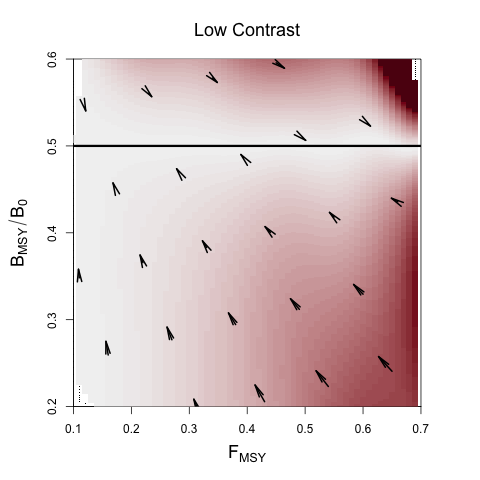
\includegraphics[width=1.1\textwidth]{../../ptNew/directionalBiasSubPTFlatT30.png}
\end{minipage}
\begin{minipage}[h!]{0.09\textwidth}
%\hspace{-1cm}
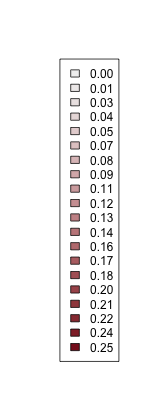
\includegraphics[width=1.5\textwidth]{../../ptNew/subLegnd.png}
\end{minipage}
%\caption{
%Joint bias direction for ($F^*$, $\frac{B^*}{B_0}$) estimates under
%the misspecified Schaefer Model. The intensity of color represents the excess
%bias relative to the shortest possible mapping. Results in the low contrast setting
%are shown $right$, and the high contrast setting is shown $left$.
%}
%\label{arrowsPT}
%\end{figure}
\end{frame}

%
\begin{frame}{Mechanism for Bias in $F_{MSY}$ via Contrast}

\only<1>{
\begin{center}
\begin{tikzpicture}[overlay]
\node at (-4.5,2) {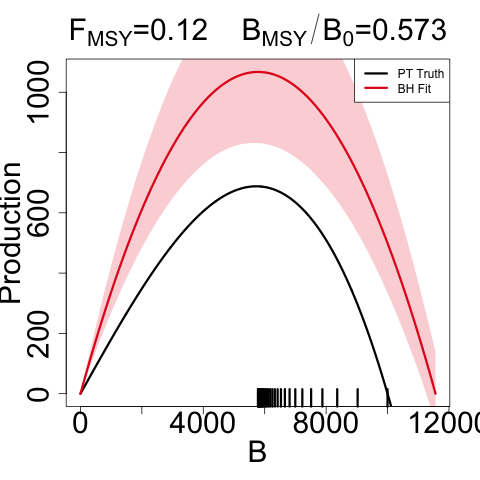
\includegraphics[width=0.2\textwidth]{../../ptNew/srrCompareFlatT30X0.12Z0.573.png}};
\node at (4.5,2) {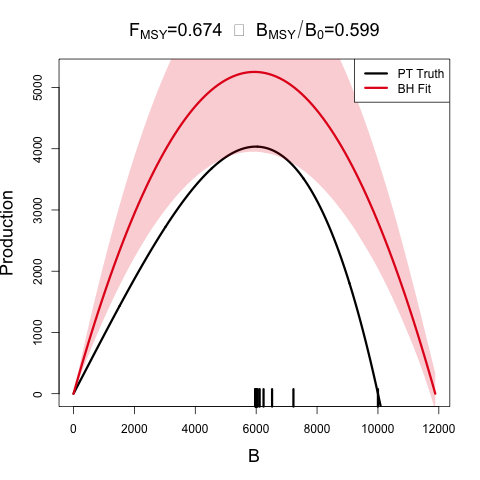
\includegraphics[width=0.2\textwidth]{../../ptNew/srrCompareFlatT30X0.674Z0.599.png}};
\node at (-4.5,-2.25) {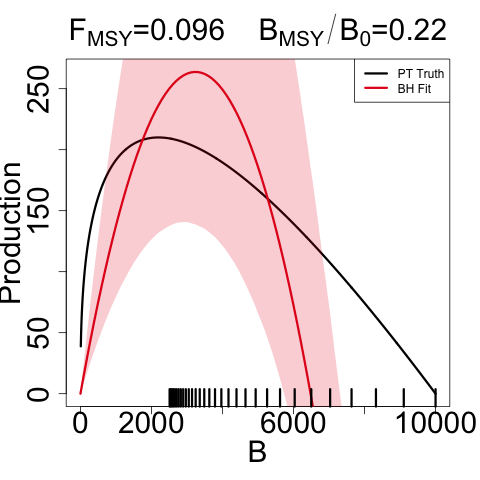
\includegraphics[width=0.2\textwidth]{../../ptNew/srrCompareFlatT30X0.096Z0.22.png}};
\node at (4.5,-2.25) {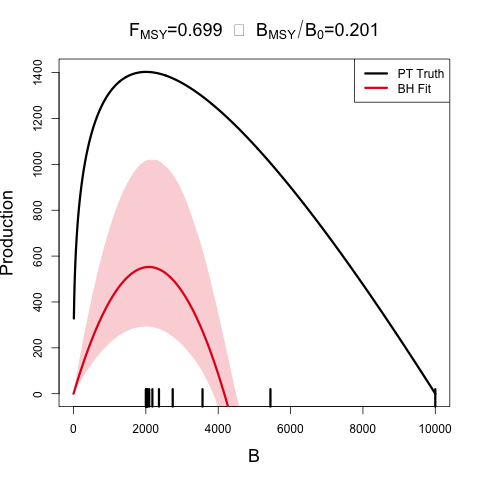
\includegraphics[width=0.2\textwidth]{../../ptNew/srrCompareFlatT30X0.699Z0.201.png}};
\node at (0,-0.5) {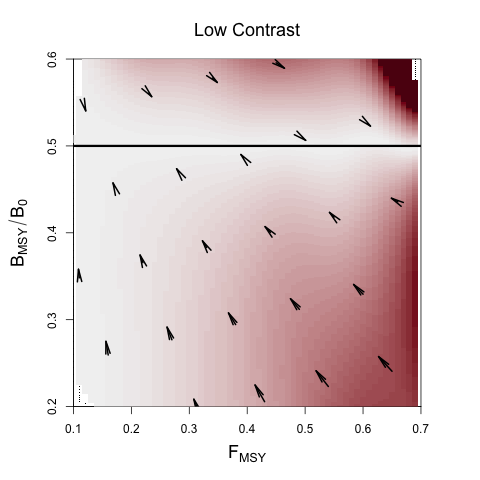
\includegraphics[width=0.65\textwidth]{../../ptNew/directionalBiasSubPTFlatT30.png}};
\end{tikzpicture}
\end{center}
}

%\begin{minipage}[h!]{0.45\textwidth}
%\begin{itemize}
%\color{red}
%\item Only observe upper half
%\item learn about slope at origin from upper biomass range
%\end{itemize}
%\end{minipage}
%\begin{minipage}[h!]{0.50\textwidth}
%\only<1>{
%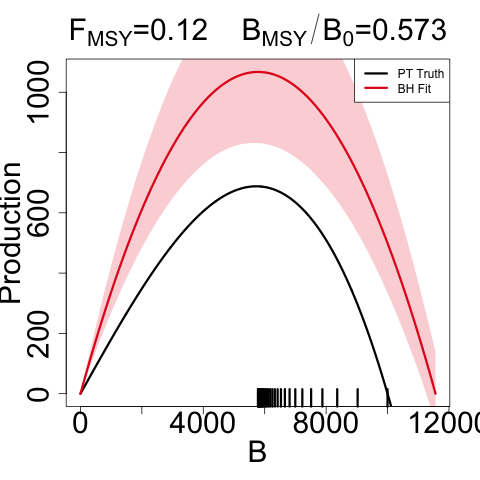
\includegraphics[width=0.47\textwidth]{../../ptNew/srrCompareFlatT30X0.12Z0.573.png}
%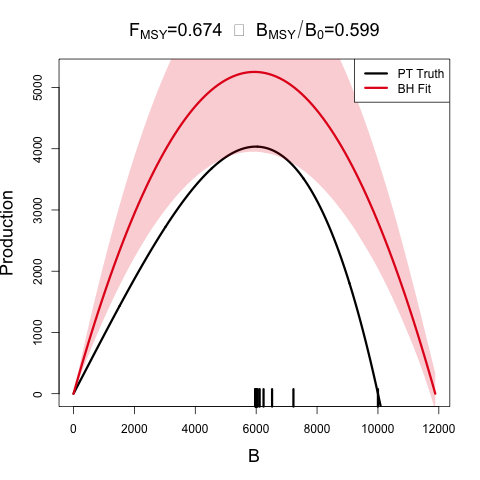
\includegraphics[width=0.47\textwidth]{../../ptNew/srrCompareFlatT30X0.674Z0.599.png}\\
%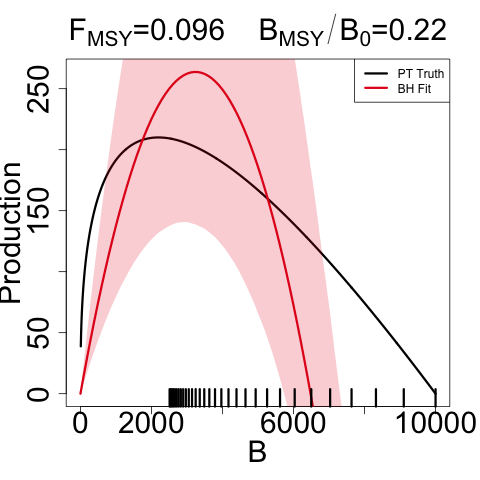
\includegraphics[width=0.47\textwidth]{../../ptNew/srrCompareFlatT30X0.096Z0.22.png}
%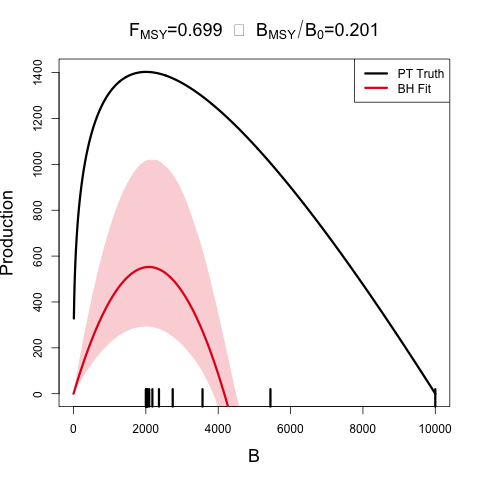
\includegraphics[width=0.47\textwidth]{../../ptNew/srrCompareFlatT30X0.699Z0.201.png}
%}

\only<2>{
\begin{minipage}[h!]{0.49\textwidth}
\begin{itemize}
%\color{red}
\setlength\itemsep{1em}
\item Low contrast limits the observation window on production. % the yeild curve observed. %Only observe upper half
%\item learn about slope at origin from upper biomass range
\item As contrast increases \\ $F^*$ bias diminishes.
\item Bias in $\frac{B^*}{B_0}$ remains, but these biases are independent of $F^*$.
%\item Under the Schaefer Model $\frac{B^*}{B_0}$ is fixed at \frac{1}{2}$; ias  but biases are independent of $F^*$.
\end{itemize}
\end{minipage}
\begin{minipage}[h!]{0.49\textwidth}
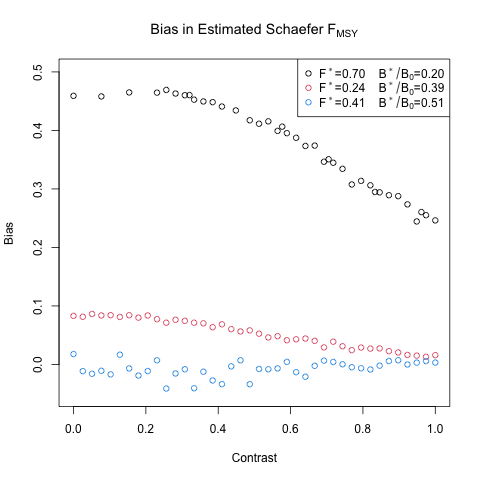
\includegraphics[width=1.1\textwidth]{../../ptNew/contrastTest3.png}
\end{minipage}
}
%\end{minipage}
\end{frame}

%%
%\begin{frame}
%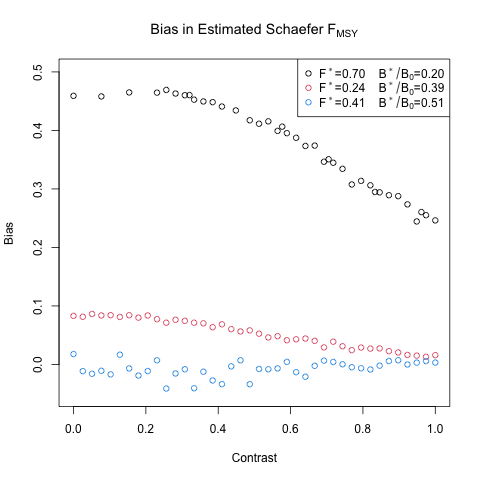
\includegraphics[width=0.5\textwidth]{../../ptNew/contrastTest3.png}
%\end{frame}

%
\begin{frame}{Summary}
\begin{itemize}
\setlength\itemsep{1em}
	%\item PT model provides a fully analytical three parameter generalization \
	\item Closed-form RP designs via three-parameter PT model. %generalization PT. %three-parameter generalization allows fully analytical \\RP designs.
	%\item Novel simulation framework explicitly controlling for \\RP misspecification. % and a useful notion of contrast.
	\item The useful notion of contrast developed here together with the simplified geometry of the 
	Schaefer model exposes a mechanism for RP bias.
	\item Metamodel describes a risk of overfishing for stocks coming from $\frac{B^*}{B_0}>\frac{1}{2}$, and overly cautious fishing for $\frac{B^*}{B_0}<\frac{1}{2}$. 
	\item What to do when the simulation design is not analytical?
\end{itemize}
\end{frame}

%
\section{The Beverton-Holt Model}
\subsection{}
\begin{frame}{Outline}
    \tableofcontents[currentsection, currentsubsection]
\end{frame}

%%
%\begin{frame}
%	\begin{minipage}[h!]{0.49\textwidth}
%	\begin{itemize}
%	\setlength\itemsep{1em}
%	\item Beverton-Holt production	
%	\item Production asymptotes
%	\item Explicit Natural Mortality
%	\item Explicit Fishing Mortality 
%	\end{itemize}
%	\end{minipage}
%	\begin{minipage}[h!]{0.49\textwidth}
%        %
%        \begin{align*}
%        I_t = q B_t e^\epsilon ~~~ \epsilon\sim N(0, \sigma^2)
%        \end{align*}
%
%        %
%        \begin{equation*}
%        \frac{dB}{dt} = P_{BH}(B(t); \bm{\theta}) -(M + F(t))B(t)
%        \end{equation*}
%	\end{minipage}
%%\begin{itemize}
%%\color{red}
%%\item Observation model
%%\item introduce logistic P
%%\item something else?
%%\end{itemize}
%\end{frame}
%
%%%
%%\begin{frame}
%%\begin{minipage}[h!]{0.49\textwidth}
%%\begin{equation*}
%%P_{BH}(B) = \frac{\alpha B}{1+\beta B}.
%%\end{equation*}
%%\begin{align}
%%F^* = 
%%\end{align}
%%\end{minipage}
%%\begin{minipage}[h!]{0.49\textwidth}
%%\end{minipage}
%%\end{frame}
%
%%
%\begin{frame}
%\begin{equation*}
%P_{BH}(B;[\alpha, \beta]) = \frac{\alpha B}{1+\beta B}.
%\end{equation*}
%\begin{align*}
%\frac{dB}{dt} = P_{BH}(B;[\alpha, \beta]) -MB -FB %(M+F)B. \label{schnuteSimple}
%\end{align*}
%\begin{minipage}[h!]{0.49\textwidth}
%        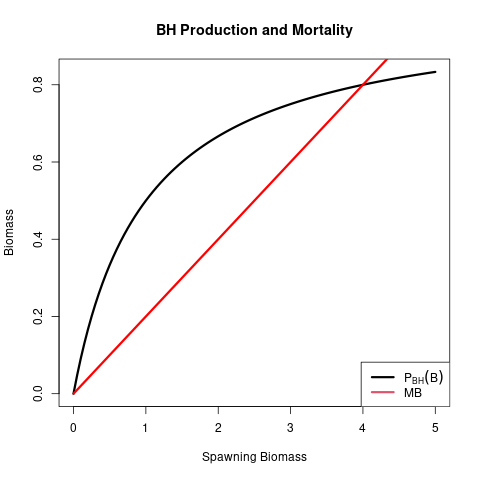
\includegraphics[width=\textwidth]{../../gpBias/pBHandM.png}
%\end{minipage}
%\begin{minipage}[h!]{0.49\textwidth}
%        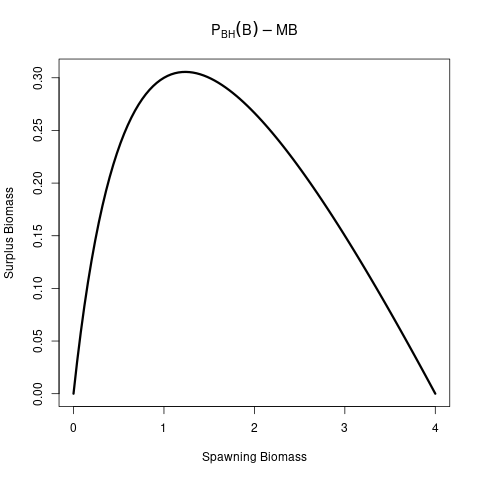
\includegraphics[width=\textwidth]{../../gpBias/yeildBH.png}
%\end{minipage}
%\end{frame}

%
\begin{frame}
\begin{minipage}[h!]{0.54\textwidth}
%
\begin{align*}
%\only<2>{&\\}
&I_t = q B_t e^\epsilon ~~~ \epsilon\sim N(0, \sigma^2)\\
%\end{align*}
%\begin{align*}
\only<1>{ &\frac{dB}{dt} = P_{BH}(B;[\alpha, \beta]) -(M+F)B\\~\\} %\underbrace{(M+F)}_{Z(t)}B\\} %(M+F)B. \label{schnuteSimple}
\only<2>{ &\frac{dB}{dt} = \underbrace{P_{BH}(B;[\alpha, \beta]) -MB}_{\text{Surplus Production}} -FB \\~\\} %~~~~\\}
\only<3>{ &\frac{dB}{dt} = \underbrace{P_{BH}(B;[\alpha, \beta]) -MB}_{\text{Surplus Production}} -FB \\~\\}
%\end{align*}
%\begin{equation*}
&\\
&P_{BH}(B;[\alpha, \beta]) = \frac{\alpha B}{1+\beta B}
\end{align*}     
\end{minipage}
\begin{minipage}[h!]{0.34\textwidth}
	\only<1>{$~$\\$~$\\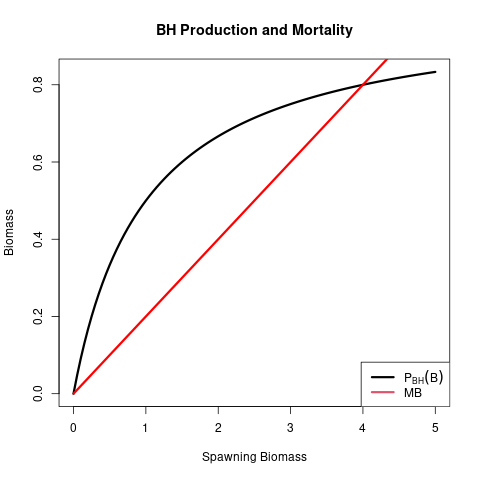
\includegraphics[width=1.5\textwidth]{../../gpBias/pBHandM.png}}
	\only<2>{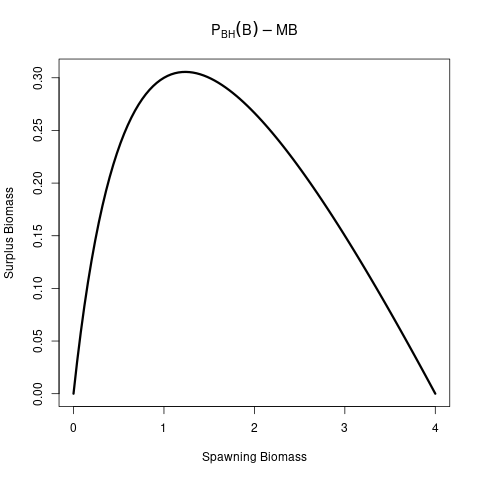
\includegraphics[width=1.5\textwidth]{../../gpBias/yeildBH.png}}
	\only<3>{
	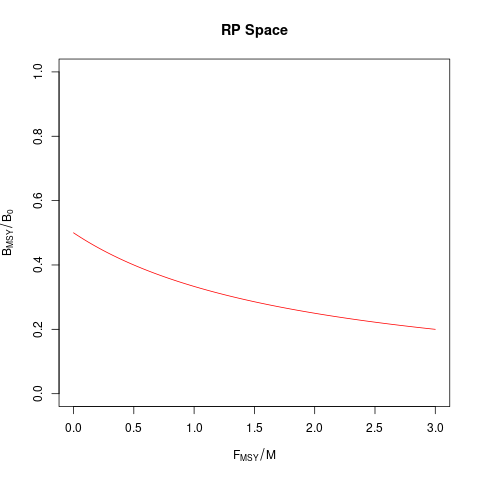
\includegraphics[width=1.5\textwidth]{bhRP.png}
	\begin{tikzpicture}[overlay]	
		\node at (3,4) { $\frac{B^*}{B_0}=\frac{1}{F^*/M+2}$ };
	\end{tikzpicture}
	}	
\end{minipage}
\end{frame}



%
\begin{frame}{Three Parameter Schnute Generalization}
\vspace{-0.25cm}
\begin{equation*}
P_s(B;[\alpha, \beta, \gamma]) = \alpha B(1-\beta\gamma B)^{\frac{1}{\gamma}}
\end{equation*}
%\vspace{-0.5cm}
%
\begin{minipage}[h!]{0.46\textwidth}
        %
        \vspace{-1cm}
        %
        \begin{center}
        {\color{Red}\underline{Logistic}}\\
        $\gamma = 1$\\$~$\\
        {\color{RoyalBlue}\underline{Ricker}}\\
        $\gamma \rightarrow 0$\\$~$\\   %\Rightarrow \text{\color{RoyalBlue}Ricker}\\   
        {\color{ForestGreen}\underline{Beverton-Holt}}\\
        $\gamma = -1$           %\Rightarrow \text{\color{ForestGreen}Beverton-Holt}\\          %\Rightarrow  \text{\color{Red}Logistic}
        \end{center}
        %
        %\begin{align*}
        %%& R(B;[\alpha, \beta, \gamma]') = \alpha B(t-a_s)(1-\beta\gamma B(t-a_s))^{\frac{1}{\gamma}}
        %%~&~\\
        %&\gamma = -1 \Rightarrow \text{\color{ForestGreen}Beverton-Holt}\\
        %&\gamma \rightarrow 0 \Rightarrow \text{\color{RoyalBlue}Ricker}\\
        %&\gamma = 1 \Rightarrow  \text{\color{Red}Logistic}
        %\end{align*}
\end{minipage}
\begin{minipage}[h!]{0.52\textwidth}	
        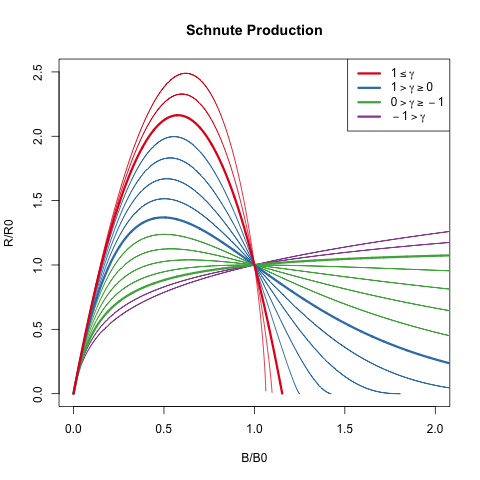
\includegraphics[width=1.1\textwidth]{../../gpBias/g3.png} %../../ddBias/designLineColorHHardFlatT30N150WWideN112.png}
\end{minipage}

%\begin{minipage}[h!]{0.49\textwidth}
%\begin{align*}
%0 &= \frac{1}{\gamma} - \left(\frac{1}{\gamma} + \frac{F^*}{F^*+M}\right)\left(\frac{F^*+M}{\alpha}\right)^\gamma\\
%\frac{B^*}{B_0} &= \frac{1-\left(\frac{M+F^*}{\alpha}\right)^\gamma}{ 1-\left(\frac{M}{\alpha}\right)^\gamma }
%\end{align*}
%\end{minipage}
%\begin{minipage}[h!]{0.49\textwidth}
%\includegraphics[width=0.65\textwidth]{../../gpBias/g3.png}
%\end{minipage}
\end{frame}

%%
%\begin{frame}
%%
%\begin{align}
%\bar{B}(F) &= \frac{1}{\gamma \beta}\left(1-\left(\frac{M+F}{\alpha}\right)^\gamma\right).
%\label{BsEq}
%\end{align}
%\begin{align}
%B_0 &= \frac{1}{\gamma \beta}\left(1-\left(\frac{M}{\alpha}\right)^\gamma\right) \label{B0S}\\
%\frac{B^*}{B_0} &= \frac{1-\left(\frac{M+F^*}{\alpha}\right)^\gamma}{ 1-\left(\frac{M}{\alpha}\right)^\gamma }. \label{BratS}
%\end{align}
%
%%
%\begin{align}
%\frac{d \bar{Y}}{dF} &= \bar B(F) + F \frac{d \bar B}{dF} \label{FderivS}\\
%\frac{d \bar B}{dF} &= -\frac{1}{\beta}  \left(\frac{\left(\frac{M+F}{\alpha}\right)^\gamma}{F+M}\right)\label{dBdFS}.
%\end{align}
%
%\begin{align}\label{FmsyS}
%0 &= \frac{1}{\gamma} - \left(\frac{1}{\gamma} + \frac{F^*}{F^*+M}\right)\left(\frac{F^*+M}{\alpha}\right)^\gamma.
%\end{align}
%\end{frame}

%
\begin{frame}{Schnute RPs Challenges}

%{\color{red}
%some how softly introduce calculation via $F^*$, $B_0$, and $\frac{B^*}{B_0}$. 
%Show the partial solution and link to Schnute and Richards citation. 
%Setup $\zeta$ for next slide.
%$\alpha(\gamma)$.
%}

%
%RPs $\mapsto$ $\theta$ or $\theta$ $\mapsto$ RPs

%%
%\begin{center}
%\begin{tikzpicture}[overlay]
%\node at (-1.5,-0.6) { RPs $\mapsto$ $\theta$ };
%\node at (0,0) {\includegraphics[height=0.15\textheight]{doubleArrow.png}};
%%\vspace*{-2cm}
%\node at (0,-0.6) {$\substack{\text{Incomplete}\\\text{Inversion}}$};
%%\vspace*{-1cm}
%\node at (0,-1) {\includegraphics[height=0.15\textheight, angle=180]{doubleArrow.png}\footnote{Schnute, J. T., \& Richards, L. J. (1998). CJFAS}};
%\node at (1.5,-0.6) { $\theta$ $\mapsto$ RPs };
%\end{tikzpicture}
%\end{center}

%
\begin{minipage}[h!]{0.44\textwidth}
%
$~$\\$~$\\
\begin{center}
\begin{tikzpicture}[overlay]
\node at (0,0.4) { RPs $\mapsto$ $\theta$ };
\node at (-1,-0.5) {\includegraphics[height=0.12\textheight, angle=90]{doubleArrow.png}};
%\vspace*{-2cm}
\node at (0,-0.5) { $\substack{\text{Incomplete}\\\text{Inversion}}$ }; %Incomplete Inversion};
%\vspace*{-1cm}
\node at (1,-0.5) {\includegraphics[height=0.12\textheight, angle=270]{doubleArrow.png}};
\node at (0,-1.6) { $\theta$ $\mapsto$ RPs };
\end{tikzpicture}
\end{center}
$~$\\$~$\\$~$\\\footnote[0]{\tiny Schnute \& Richards (1998). CJFAS.}
%
\end{minipage}
\begin{minipage}[h!]{0.54\textwidth}
%
\only<1>{
\begin{align*}
%\frac{B^*}{B_0} &= \frac{1-\left(\frac{M+F^*}{\alpha}\right)^\gamma}{ 1-\left(\frac{M}{\alpha}\right)^\gamma } \\
\alpha &= (M+F^*)\left(1+\frac{\gamma F^*}{M+F^*}\right)^{1/\gamma} \nonumber\\
\beta &= \frac{1}{\gamma B_0}\left(1-\left(\frac{M}{\alpha}\right)^\gamma\right) \label{abgSys}\\
\frac{B^*}{B_0} &= \frac{1-\left(\frac{M+F^*}{\alpha}\right)^\gamma}{ 1-\left(\frac{M}{\alpha}\right)^\gamma } \nonumber.
\end{align*}
}
\only<2>{
\begin{align*}
&\alpha(\gamma)\\
&\\
&\beta(\alpha(\gamma), \gamma)\\
&\\
&\frac{B^*}{B_0}(\alpha(\gamma),\gamma)
\end{align*}
}
%\end{frame}
%
\end{minipage}
\end{frame}


%
\begin{frame}{Sudo Inverse Inverse-CDF Sampling}
%{\color{red}
%Show approximated $t$ with rugs. explain/relabel $\zeta$. show qq plot.
%}

%\begin{align}
%\gamma' \sim \zeta_{min}\delta(\gamma_{min}) + t(\mu, \sigma, \nu)\bm{1}_{\gamma>\gamma_{min}}
%\end{align}
%\includegraphics[width=0.5\textwidth]{../../gpBias/zeta.png}
%\end{frame}
%%
%\begin{frame}

%
\begin{minipage}[h!]{0.54\textwidth}
$~$\\
\hspace*{-2cm}
\begin{align*}
\frac{B^*}{B_0}(\gamma) = \frac{1-\left(\frac{M+F^*}{\alpha(\gamma)}\right)^\gamma}{ 1-\left(\frac{M}{\alpha(\gamma)}\right)^\gamma }
\end{align*}
\only<1>{
\begin{align*}
~
\end{align*}
}
\only<2>{
\begingroup
\scriptsize
{\color{RoyalBlue}
\begin{align*}
\gamma' \sim \zeta_{min}\delta(\gamma_{min}) + (1-\zeta_{min})t(\mu, \sigma, \nu)\bm{1}_{\gamma>\gamma_{min}}
\end{align*}
}
\endgroup
}
\only<3>{
\begingroup
\scriptsize
{\color{RoyalBlue}
\begin{align*}
\gamma' \sim \zeta_{min}\delta(\gamma_{min}) + (1-\zeta_{min})t(\mu, \sigma, \nu)\bm{1}_{\gamma>\gamma_{min}}
\end{align*}
}
\endgroup
}
\end{minipage}
\begin{minipage}[h!]{0.44\textwidth}
\only<1>{\includegraphics[width=1.2\textwidth]{../../gpBias/zetaTitle.png}}
\only<2>{\includegraphics[width=1.2\textwidth]{../../gpBias/zetaPlusPlus.png}}
\only<3>{\includegraphics[width=1.2\textwidth]{../../gpBias/qqUnif.png}}
\end{minipage}
\end{frame}



%animate between curve picture to RP curves
%\begin{frame}{Schnute LHS Design}
%%%
%%\vspace{-0.25cm}
%%\begin{equation*}
%%R(B;\alpha, \beta, \gamma) = \alpha B_{t-a_s}(1-\beta\gamma B_{t-a_s})^{\frac{1}{\gamma}}
%%\end{equation*}
%\begin{equation*}
%P_s(B;[\alpha, \beta, \gamma]) = \alpha B(1-\beta\gamma B)^{\frac{1}{\gamma}}
%\end{equation*}

%
\begin{frame}{Schnute LHS Design}
%
\begin{minipage}[h!]{0.54\textwidth}
        %
        \vspace{-1cm}
        %
	\only<1>{
        \begin{center}
        {\color{Red}\underline{Logistic}}\\
        $\gamma = 1$\\$~$\\
        {\color{RoyalBlue}\underline{Ricker}}\\
        $\gamma \rightarrow 0$\\$~$\\   %\Rightarrow \text{\color{RoyalBlue}Ricker}\\   
        {\color{ForestGreen}\underline{Beverton-Holt}}\\
        $\gamma = -1$           %\Rightarrow \text{\color{ForestGreen}Beverton-Holt}\\          %\Rightarrow  \text{\color{Red}Logistic}
        \end{center}
	}
	%
	\only<2>{
	$~$\\$~$\\$~$\\$~$\\
	\begingroup
	\scriptsize
	\begin{equation*}
	\underbrace{\left(\frac{F_{MSY}}{M}, \frac{B_{MSY}}{\bar B(0)}\right)}_{\text{Schnute Truth}} {\text{GP}\atop{\mapsto\atop~}} \underbrace{\left(\frac{\hat F_{MSY}}{M}, \frac{1}{\hat F_{MSY}/M+2}\right)}_{\text{BH Estimate}}
	\end{equation*}
	\endgroup
	}
%\hspace{-1cm}

%\end{minipage}
%\begin{minipage}[h!]{0.39\textwidth}
%\begin{center}
%\begin{tikzpicture}[overlay]
%\only<1>{
%\node at (0.5,0) {\includegraphics[height=0.65\textheight]{../../ptNew/simplePTDesign.png}};%gpBias/designLineHHardExpT45N150M0.3Wide.png}};	
        %
        %\begin{align*}
        %%& R(B;[\alpha, \beta, \gamma]') = \alpha B(t-a_s)(1-\beta\gamma B(t-a_s))^{\frac{1}{\gamma}}
        %%~&~\\
        %&\gamma = -1 \Rightarrow \text{\color{ForestGreen}Beverton-Holt}\\
        %&\gamma \rightarrow 0 \Rightarrow \text{\color{RoyalBlue}Ricker}\\
        %&\gamma = 1 \Rightarrow  \text{\color{Red}Logistic}
        %\end{align*}
\end{minipage}
\begin{minipage}[h!]{0.44\textwidth}
        \only<1>{
	\includegraphics[height=0.7\textheight]{../../ddBias/designLineColorHHardFlatT30N150WWideN112.png}}
	\only<2>{
	%\begin{center}
	$~$\\
	\begin{tikzpicture}[overlay]
	\node at (2.75,0) {\includegraphics[height=0.7\textheight]{../../gpBias/designLineHHardExpT45N150M0.3Wide.png}};
	\node[circle, draw, minimum size=7, inner sep=-2] at (4.35,1.5){\tiny S};
	\draw[latex-, very thick,black] (2.35,-0.9) -- ++(1.9,2.3);
	\node[circle,fill=red, minimum size=9, inner sep=-2] at (2.25,-1){\tiny BH};
	\end{tikzpicture}
	%\end{center}
	%\includegraphics[width=1.1\textwidth]{../../gpBias/designLineHHardExpT45N150M0.3Wide.png}
	}
\end{minipage}
\end{frame}


%%
%\begin{frame}
%%\begin{figure}[h!]
%\begin{minipage}[h!]{0.46\textwidth}
%\hspace*{0.5cm}
%%\includegraphics[width=1.175\textwidth]{../../gpBias/zetaRelBiasSchnuteExpT45N150Wide.png}\\
%\includegraphics[height=0.49\textheight]{../../gpBias/zetaRelBiasSchnuteExpT45N150Wide.png}\\
%\hspace*{1cm}
%\vspace{-1cm}
%%\caption{\label{contrastTrio}
%%Heatplots showing the bias in RP estimation induced by model misspecification of
%%the BH model in the high contrast simulation setting.
%%In all cases the restricted RP-space of the BH set is shown as the black curve.
%%(\emph{left}) Relative bias in $\frac{B^*}{\bar B(0)}$.  (\emph{top-right})
%%Bias in RP-space shown directionally. Arrows point from the location where
%%data is generated, toward the location in the BH set where MLE projects estimated
%%RPs. The intensity of color represents the excess bias relative
%%to the shortest possible mapping. (\emph{bottom}) Relative bias in $\frac{F^*}{M}$.
%%}
%$~$\\$~$\\$~$\\$~$\\$~$\\$~$\\$~$\\$~$\\$~$\\
%\end{minipage}
%\begin{minipage}[h!]{0.44\textwidth}
%$~$\\
%\vspace{-1cm}
%\hspace*{-0.1cm}
%\includegraphics[height=0.49\textheight]{../../gpBias/directionalBiasSchnuteSubTitleExpT45N150Wide.png}\\
%$~$\\$~$\\
%\hspace*{0.1cm}
%\includegraphics[height=0.49\textheight]{../../gpBias/fMSYRelBiasSchnuteExpT45N150Wide.png}
%\end{minipage}
%\begin{minipage}[h!]{0.07\textwidth}
%\vspace{-4cm}
%\hspace*{-1.25cm}
%\includegraphics[width=1.5\textwidth]{../../gpBias/legendSubSchnute.png}
%\end{minipage}
%%\end{figure}
%\end{frame}


%
\begin{frame}
\only<1>{
\begin{center}
\begin{tikzpicture}[overlay]
        \node at (0.25,-0.5) {\includegraphics[height=0.92\textheight]{../../gpBias/directionalBiasSchnuteSubTitleExpT45N150Wide.png}};
        %\node at (4.5,2)  {\includegraphics[scale=0.15]{../gpBias/yeildCurveTruthExpT45N150WideX3.348Z0.541.png}};
        %\node at (-4.75,-2.5)  {\includegraphics[scale=0.15]{../gpBias/yeildCurveFitExpT45N150WideX3.348Z0.541.png}};
\end{tikzpicture}
\end{center}
}
\only<2>{
\begin{center}
\begin{tikzpicture}[overlay]
        \node at (0.25,-0.5) {\includegraphics[height=0.92\textheight]{../../gpBias/directionalBiasSchnuteSubTitleExpT45N150Wide.png}};
        \node at (4.75,0)  {\includegraphics[scale=0.18]{../../gpBias/yeildCurveTruthExpT45N150WideX2.5Z0.45.png}}; 
	\node at (1.25,0) [circle,fill,inner sep=1.75pt]{};
	%\node at (-4.75,-2.5)  {\includegraphics[scale=0.15]{../gpBias/yeildCurveFitExpT45N150WideX3.348Z0.541.png}};
\end{tikzpicture}
\end{center}
}
\only<3>{
\begin{center}
\begin{tikzpicture}[overlay]
        \node at (0.25,-0.5) {\includegraphics[height=0.92\textheight]{../../gpBias/directionalBiasSchnuteSubTitleExpT45N150Wide.png}};
        \node at (4.75,0)  {\includegraphics[scale=0.18]{../../gpBias/yeildCurveTruthExpT45N150WideX2.5Z0.45.png}};
        \node at (-4.75,-2.25)  {\includegraphics[scale=0.18]{../../gpBias/yeildCurveFitExpT45N150WideX2.5Z0.45.png}};
        \node at (1.25,0) [circle,fill,inner sep=1.75pt]{};
        \node at (-0.35,-2) [circle,fill=red,inner sep=1.75pt]{};
\end{tikzpicture}
\end{center}
}
\end{frame}

%
\begin{frame}
\only<1>{
\begin{center}
\begin{tikzpicture}[overlay]
        \node at (0.25,-0.5) {\includegraphics[height=0.92\textheight]{../../gpBias/directionalBiasSchnuteSubSpaceHHardFlatT30N150WWideN112.png}};
        %\node at (4.5,2)  {\includegraphics[scale=0.15]{../gpBias/yeildCurveTruthExpT45N150WideX3.348Z0.541.png}};
        %\node at (-4.75,-2.5)  {\includegraphics[scale=0.15]{../gpBias/yeildCurveFitExpT45N150WideX3.348Z0.541.png}};
\end{tikzpicture}
\end{center}
}
\only<2>{
\begin{center}
\begin{tikzpicture}[overlay]
        \node at (0.25,-0.5) {\includegraphics[height=0.92\textheight]{../../gpBias/directionalBiasSchnuteSubSpaceHHardFlatT30N150WWideN112.png}};
        \node at (4.75,0)  {\includegraphics[scale=0.18]{../../gpBias/yeildCurveTruthHHardFlatT30N150WWideN112X3Z0.55.png}}; %{\includegraphics[scale=0.18]{../../gpBias/yeildCurveTruthExpT45N150WideX2.5Z0.45.png}}; 
	\node at (2,1.4) [circle,fill=white,inner sep=2pt]{};
	\node at (2,1.4) [circle,fill,inner sep=1.75pt]{};
	%\node at (-4.75,-2.5)  {\includegraphics[scale=0.15]{../gpBias/yeildCurveFitExpT45N150WideX3.348Z0.541.png}};
\end{tikzpicture}
\end{center}
}
\only<3>{
\begin{center}
\begin{tikzpicture}[overlay]
        \node at (0.25,-0.5) {\includegraphics[height=0.92\textheight]{../../gpBias/directionalBiasSchnuteSubSpaceHHardFlatT30N150WWideN112.png}};
        \node at (4.75,0)  {\includegraphics[scale=0.18]{../../gpBias/yeildCurveTruthHHardFlatT30N150WWideN112X3Z0.55.png}}; %{\includegraphics[scale=0.18]{../../gpBias/yeildCurveTruthExpT45N150WideX2.5Z0.45.png}};
        \node at (-4.75,-2.25)  {\includegraphics[scale=0.18]{../../gpBias/yeildCurveFitHHardFlatT30N150WWideN112X3Z0.55.png}}; %{\includegraphics[scale=0.18]{../../gpBias/yeildCurveFitExpT45N150WideX2.5Z0.45.png}};
        \node at (2,1.4) [circle,fill=white,inner sep=2pt]{};
        \node at (2,1.4) [circle,fill,inner sep=1.75pt]{};
	\node at (-2,0.4) [circle,fill=red,inner sep=1.75pt]{};
	%\node at (1.25,0) [circle,fill=white,inner sep=2pt]{};
	%\node at (1.25,0) [circle,fill,inner sep=1.75pt]{}; 
	%\node at (-0.35,-2) [circle,fill=red,inner sep=1.75pt]{};
\end{tikzpicture}
\end{center}
}
\only<4>{
\begin{center}
\begin{tikzpicture}[overlay]
        \node at (0.25,-0.5) {\includegraphics[height=0.92\textheight]{../../gpBias/directionalBiasSchnuteSubSpaceHHardFlatT30N150WWideN112.png}}; %{\includegraphics[height=0.92\textheight]{../../gpBias/directionalBiasSchnuteAnimateSourceHHardFlatT30N150WWideN112X3Z0.35.png}};
        \node at (4.75,-1)  {\includegraphics[scale=0.18]{../../gpBias/yeildCurveTruthHHardFlatT30N150WWideN112X3Z0.35.png}};
        \node at (2.15,-0.9) [circle,fill=white,inner sep=2pt]{};
        \node at (2.15,-0.9) [circle,fill,inner sep=1.75pt]{};
	%\node at (-4.75,-2.5)  {\includegraphics[scale=0.15]{../gpBias/yeildCurveFitHHardFlatT30N150WWideN56X3.497Z0.578.png}};
\end{tikzpicture}
\end{center}
}
\only<5>{
\begin{center}
\begin{tikzpicture}[overlay]
        \node at (0.25,-0.5) {\includegraphics[height=0.92\textheight]{../../gpBias/directionalBiasSchnuteSubSpaceHHardFlatT30N150WWideN112.png}}; %\includegraphics[height=0.92\textheight]{../../gpBias/directionalBiasSchnuteAnimateSinkHHardFlatT30N150WWideN112X3Z0.35.png}};
        \node at (4.75,-1)  {\includegraphics[scale=0.18]{../../gpBias/yeildCurveTruthHHardFlatT30N150WWideN112X3Z0.35.png}};
        \node at (-4.75,-2.25)  {\includegraphics[scale=0.18]{../../gpBias/yeildCurveFitHHardFlatT30N150WWideN112X3Z0.35.png}};
	\node at (2.15,-0.9) [circle,fill=white,inner sep=2pt]{};
        \node at (2.15,-0.9) [circle,fill,inner sep=1.75pt]{};
	\node at (0.45,-2.2) [circle,fill=red,inner sep=1.75pt]{};
\end{tikzpicture}
\end{center}
}
%\only<6>{
%\begin{center}
%\begin{tikzpicture}[overlay]
%        \node at (0.25,-0.5) {\includegraphics[height=0.92\textheight]{../../gpBias/directionalBiasSchnuteSubSpaceHHardFlatT30N150WWideN112.png}}; %\includegraphics[height=0.92\textheight]{../../gpBias/directionalBiasSchnuteAnimateSinkHHardFlatT30N150WWideN112X3Z0.35.png}};
%        \node at (4.75,-1)  {\includegraphics[scale=0.18]{../../gpBias/yeildCurveTruthHHardFlatT30N150WWideN112X3Z0.35.png}};
%        \node at (-4.75,-2.25)  {\includegraphics[scale=0.18]{../../gpBias/yeildCurveFitHHardFlatT30N150WWideN112X3Z0.35.png}};
%        \draw[very thick,blue] (-2.25,0.5) -- ++(5.25,-1.1);
%	\node at (2.15,-0.9) [circle,fill=white,inner sep=2pt]{};
%        \node at (2.15,-0.9) [circle,fill,inner sep=1.75pt]{};
%        \node at (0.45,-2.2) [circle,fill=red,inner sep=1.75pt]{};
%\end{tikzpicture}
%\end{center}
%}
\end{frame}

%
\begin{frame}
\begin{minipage}[h!]{0.49\textwidth}
        \includegraphics[width=1\textwidth]{../../gpBias/directionalBiasSchnuteSubHHardFlatT30N150WWideN112.png}
\end{minipage}
\begin{minipage}[h!]{0.49\textwidth}
        \includegraphics[width=1\textwidth]{../../ddBias/designLineColorHHardFlatT30N150WWideN112.png}
\end{minipage}
\end{frame}

\begin{frame}{Summary}
%\color{red}Quick Summary and Transition
\begin{itemize}
\setlength\itemsep{1em}
        %\item PT model provides a fully analytical three parameter generalization \
        \item Schnute three-parameter generalizing model is very attractive since it  
	interpolates the most common models of productivity. 
	\begin{itemize}
		\item Logistic, Ricker, Beverton-Holt
	\end{itemize}
	%however simulation design is not analytical and numerically trechreous. %  allows fully analytical \\RP designs.        \item Novel simulation framework explicitly controlling for \\RP misspecification. % and a useful notion of contrast.
        \item A stable method of generating simulation designs despite non-analytical 
	and numerically treacherous RPs$\leftrightarrow\theta$.	
	\item GP metamodel demonstrates that misspecified BH models enjoy some sense of optimality in RP estimation.
	\begin{itemize}
	 	\item Nearly shortest distance RP mapping as mediated by contrast.
		\item but misspecified BH models induce a risk structure in RPs.
	\end{itemize}
	\item Can more complex biological dynamics help RP estimation?
\end{itemize}

\end{frame}

%
\section{Delay Differential Growth Extension}
\subsection{}
\begin{frame}{Outline}
    \tableofcontents[currentsection, currentsubsection]
\end{frame}

%
\begin{frame}{General Modeling Structure}
\begin{align*}%\kappa->0 slower that than a0->\infty
%B(a, t) &= w(a, t)N(a, t)\\ 
%\frac{dB}{dt} &= \overbrace{w(k)R(B(t-k))}^\text{Recruitment Biomass} + \overbrace{\mu w_\infty N(t)}^\text{Growth} - \overbrace{(M+F(t)+\mu)B(t)}^\text{Biomass Loss}\\
&I_t = q B_t e^\epsilon ~~~ \epsilon\sim N(0, \sigma^2)\\
&\\
&\frac{dB}{dt} = \overbrace{w(a_s)R(B;\theta)}^\text{Recruitment Biomass} + \overbrace{\kappa \left[w_\infty N-B\right]}^\text{Net Growth} - \overbrace{(M+F)B}^\text{Mortality} \\%\label{
&\frac{dN}{dt} = R(B;\theta) - (M+F)N \\%\label{nEq}\\
%&~\\
%&R(B_{t-a_s}; \alpha, \beta, \gamma): \text{Schnute Three Parameter Recruitment}\\
%&w(a) : \text{Von Bertalanffy Individual Growth}\\
%&\text{Knife-Edge Selectivity at age $a_s$}\\
%&\theta' = [\alpha, \beta, \gamma] ~~~ ~~~ {\color{Red} \text{Species Properties: } a_0,~\kappa,~w_\infty,~M}
\end{align*}
%{\color{red} bullets of primary points of individual growth and maturity}
\footnote[0]{\tiny Walters, C. J. (2020). The continuous time Schnute-Deriso delay difference model for age-structured population dynamics, with example application to the Peru anchoveta stock. University of British Columbia.}
\end{frame}

%
\begin{frame}{Individual Growth}
%
\begin{minipage}[h!]{0.47\textwidth}
        %
        \vspace{-1cm}
        \begin{align*}
        w(a) = w_\infty(1-e^{-\kappa (a-a_0)}) %\\
        \end{align*}
	%$a_s$ : Lagged Maturity/Knife-edge Selectivity\\
        %$~\kappa$ : Individual Growth
        \vspace*{-0.25cm}
        \begin{itemize}
	\setlength\itemsep{1em}
        \item[$a_s$ :] Lagged Maturity \&\\Knife-Edge Selectivity
	\item[$\kappa$ :] Individual Growth
	\item Instant Growth: \\(Production Model)\\
        %\begin{align*}
        $a_s \rightarrow 0 ~~~ \kappa \rightarrow \infty$\\$~$\\
        %\end{align*}
        %\item Dynamic Growth:\\
        %%$a_s$ large relative to $\kappa$\\
        %$a_s$ : Not Instant\\
        %$~\kappa$ : Peakness of Dynamics
        \end{itemize}
        %{\color{red}
        %limiting cases as prod model\\
        %knife edge selectivity\\
        %animate to RP space curve under BH.
        %}
\end{minipage}
\begin{minipage}[h!]{0.51\textwidth}
	\only<1>{
        \includegraphics[width=1.1\textwidth]{../plots/vbOpt.png}
	}
	\only<2>{
        \includegraphics[width=1.1\textwidth]{../../ddBias/vbCurves.png}
	}
	%\includegraphics[width=0.49\textwidth]{../../ddBias/rpTriptic.png}
	%\includegraphics[width=0.49\textwidth]{../../ddBias/growthTriptic.png}
\end{minipage}
\end{frame}

%%
%\begin{frame}{Growth}
%
%\end{frame}

%animate between curve picture to RP curves
\begin{frame}{Schnute Recruitment}
%
\vspace{-0.25cm}
\begin{equation*}
R(B;\alpha, \beta, \gamma) = \alpha B_{t-a_s}(1-\beta\gamma B_{t-a_s})^{\frac{1}{\gamma}}
\end{equation*}
%
\begin{minipage}[h!]{0.46\textwidth}
        %
        \vspace{-1cm}
        %
        \begin{center}
        {\color{Red}\underline{Logistic}}\\
        $\gamma = 1$\\$~$\\
        {\color{RoyalBlue}\underline{Ricker}}\\
        $\gamma \rightarrow 0$\\$~$\\   %\Rightarrow \text{\color{RoyalBlue}Ricker}\\   
        {\color{ForestGreen}\underline{Beverton-Holt}}\\
        $\gamma = -1$           %\Rightarrow \text{\color{ForestGreen}Beverton-Holt}\\          %\Rightarrow  \text{\color{Red}Logistic}
        \end{center}
        %
        %\begin{align*}
        %%& R(B;[\alpha, \beta, \gamma]') = \alpha B(t-a_s)(1-\beta\gamma B(t-a_s))^{\frac{1}{\gamma}}
        %%~&~\\
        %&\gamma = -1 \Rightarrow \text{\color{ForestGreen}Beverton-Holt}\\
        %&\gamma \rightarrow 0 \Rightarrow \text{\color{RoyalBlue}Ricker}\\
        %&\gamma = 1 \Rightarrow  \text{\color{Red}Logistic}
        %\end{align*}
\end{minipage}
\begin{minipage}[h!]{0.52\textwidth}
        %\only<1>{
        \includegraphics[width=1.1\textwidth]{../../gpBias/g3.png} %./derisoSrr.png}
        %}
	%\only<2>{
        %\includegraphics[width=1.1\textwidth]{../../ddBias/designLineColorHHardFlatT30N150WWideN112.png}
        %}
\end{minipage}
\end{frame}

%%NOTE: RP Space
%\begin{frame}
%\includegraphics[width=0.54\textwidth]{../../ddBias/rpSpaceww.png}
%\end{frame}

%
\begin{frame}{Growth Further Complicates RPs}
%%
%\begin{align}
%\bar{B}(F) &= \frac{1}{\beta\gamma} \left( 1 - \Big(\frac{(F + M) (F + M + \kappa)}{\alpha w(a_s)(F + M + \kr)}\Big)^\gamma\right) \label{BF}\\
%%\end{align}
%%\begin{align}
%\bar{N}(F) &= \frac{\alpha\bar{B}(F)(1-\beta\gamma\bar{B}(F))^{1/\gamma}}{F+M} \label{NF}
%\end{align}

%\begingroup
%\tiny
%\begin{align}
%\frac{d \bar{Y}}{dF} &= \frac{1}{\beta\gamma}\left[ 1 - \one - \two \left( 1 + \thr \right) \right]\label{dBdFS}
%%&= (1-\left(\frac{(F+M)*(F+M+\kappa)}{\alpha*(F*w(a_s)+M*w(a_s)+\kappa*w_infty)}\right)^\gamma-(F*(((F+M)*(F+M+\kappa))/(\alpha*(F*w(a_s)+M*w(a_s)+\kappa
%%&= ( 1-\Big(\frac{(F+M)(F+M+\kappa)}{\alpha w(a_s)(F+M+\kappa w_\infty/w(a_s))}\Big)^\gamma - ( F*( ((F+M)*(F+M+\kappa))/(\alpha*(F*w(a_s)+M*w(a_s)+\kapp
%\end{align}
%\endgroup

%
\begingroup
\tiny
\begin{gather*}
~~~~ \alpha  = \left[ \oneA + \twoA \left( 1 + \thrA \right) \right]^{\frac{1}{\gamma}} \label{aDelay}\\ ~\\
\beta = \frac{1}{\gamma B_0} \left( 1 - \Big(\frac{M (M + \kappa)}{\alpha w(a_s)(M + \kr)}\Big)^\gamma\right) \\ ~\\
%\frac{B^*}{B_0} &= \frac{ 1 - \Big(\frac{(F^* + M) (F^* + M + \kappa)}{\alpha w(a_s)(F^* + M + \kr)}\Big)^\gamma }{ 1 - \Big(\frac{M (M + \kappa)}{\alpha
%\end{align*}
%\endgroup
%\begin{align}
\frac{B^*}{B_0} = \frac{ 1 - \Big(\frac{(F^* + M) (F^* + M + \kappa)}{\alpha w(a_s)(F^* + M + \kr)}\Big)^\gamma }{ 1 - \Big(\frac{M (M + \kappa)}{\alpha w(a_s)(M + \kr)}\Big)^\gamma }
%\label{gDelay}
\end{gather*}
\endgroup


%\begin{align*}
%&\alpha(\gamma)\\
%&\\
%&\beta(\alpha(\gamma), \gamma)\\
%&\\
%&\frac{B^*}{B_0}(\alpha(\gamma),\gamma)
%\end{align*}
%-5.85
%-3.5
\begin{center}
\begin{tikzpicture}[overlay]
\node at (-5.65,3.95) { $\alpha(\gamma):$ };
\node at (-5.4,2.65) { $\beta(\alpha(\gamma), \gamma):$ };
\node at (-5.3,1.2) { $\frac{B^*}{B_0}(\alpha(\gamma), \gamma):$ };
\end{tikzpicture}
\end{center}

\end{frame}


%
\begin{frame}
\only<1>{ \includegraphics[width=0.49\textwidth]{../../gpBias/zetaPlusPlus.png} }
\only<2>{ \includegraphics[width=0.49\textwidth]{../../gpBias/zetaPlusPlus.png} }
%
\only<3>{
        $~$\\
        \begingroup
        \scriptsize
        \begin{equation*}
        \underbrace{\left(\frac{F^*}{M}, \frac{B^*}{\bar B(0)}\right)}_{\text{Schnute Truth}} {\text{GP}\atop{\mapsto\atop~}} \underbrace{\left(\frac{\hat F^*}{M}, \frac{B^*}{B_0}(-1; \hat F^*)\right)}_{\text{BH Estimate}}~~~~~~~~~~~~~~~~~~~~~~~~~~~~~~~~~~~~~~~~~~~~~~~~~~~~~~~~~~~~~~~~~~~~~~~~~~~~~~~~~~~~~~~~~~
        \end{equation*}
        \endgroup
}

 \begin{tikzpicture}[overlay]
        \only<2>{{\node at (8.5,3.45) {\includegraphics[height=0.7\textheight]{../../gpBias/designLineHHardExpT45N150M0.3Wide.png}};}}
	\only<3>{{\node at (8.5,1.75) {\includegraphics[height=0.7\textheight]{../../gpBias/designLineHHardExpT45N150M0.3Wide.png}};}}
	\only<3>{
        \node[circle, draw, minimum size=7, inner sep=-2] at (10.1,3.25){\tiny S};
        \draw[latex-, very thick,black] (8.1,0.85) -- ++(1.9,2.3);
        \node[circle,fill=red, minimum size=9, inner sep=-2] at (8.0,0.72){\tiny BH};
	}
\end{tikzpicture}
%\includegraphics[width=0.49\textwidth]{../../gpBias/zetaPlusPlus.png}
\end{frame}

%
\begin{frame}{High Contrast}
	\begin{minipage}[h!]{0.51\textwidth}
	%
	\includegraphics[width=\textwidth]{../../ddBias/vbPoster.png}
	\end{minipage}
	\begin{minipage}[h!]{0.47\textwidth}
	\centering
	\vspace{-0.25cm}
	\includegraphics[height=0.28\textheight]{../../ddBias/directionalBiasDDSubExpT45N300AS0.1K10PresReds 2.png}\\ %directionalBiasDDSubFlatT45N150A0-1AS0.1K10N56Reds 2.png}\\
        \includegraphics[height=0.28\textheight]{../../ddBias/directionalBiasDDSubExpT45N150A0-1AS4K0.2N38Purples.png}\\ %directionalBiasDDSubFlatT45N150A0-1AS1K0.5N56Purples.png}\\
	%\hspace{0.05cm}directionalBiasDDSubExpT45N150A0-1AS2K0.1Reds 2.png
	\includegraphics[height=0.28\textheight]{../../ddBias/directionalBiasDDSubExpT45N150A0-1AS2K0.1Blues.png} %directionalBiasDDSubExpT45N150A0-1AS2K0.1Reds 2.png}
	%%
	%\includegraphics[width=0.32\textwidth]{../../ddBias/directionalBiasDDSubFlatT45N150A0-1AS0.1K10N56Reds 2.png}
        %\includegraphics[width=0.32\textwidth]{../../ddBias/directionalBiasDDSubFlatT45N150A0-1AS1K0.5N56Purples.png}
        %\includegraphics[width=0.32\textwidth]{../../ddBias/directionalBiasDDSubFlatT45N150A0-1AS2K0.1N84EdgeBlues.png}	
	\end{minipage}
\end{frame}

%
\begin{frame}{Low Contrast}
	\begin{minipage}[h!]{0.51\textwidth}
	%
	\includegraphics[width=\textwidth]{../../ddBias/vbPoster.png}
	\end{minipage}
	\begin{minipage}[h!]{0.47\textwidth}
	%
	\centering
	\only<1>{
	\vspace{-0.25cm}
	\includegraphics[height=0.28\textheight]{../../ddBias/directionalBiasDDSubFlatT45N150A0-1AS0.1K10N56PresReds 2.png}\\
        \includegraphics[height=0.28\textheight]{../../ddBias/directionalBiasDDSubFlatT45N150A0-1AS1K0.5N56Purples.png}\\
	\hspace{0.1cm}
	\includegraphics[height=0.28\textheight]{../../ddBias/directionalBiasDDSubFlatT45N150A0-1AS2K0.1N84EdgeBlues.png}
	}
	\only<2>{
	$~$\\
	\vspace*{0.3cm}	
	\includegraphics[width=\textwidth]{../../ddBias/relErrorImagesBHDD0.5.png}
	}
	\end{minipage}
\end{frame}

%
\begin{frame}{Oscillation}
	%\centering
        \begin{minipage}[h!]{0.39\textwidth}
	\begin{itemize}
        \setlength\itemsep{1em}
	\item Large $a_s$ window.
	\item Fishing shocks \\within $a_s$ window.
	\item Repeated shocks \\can lead to chaos.
	\end{itemize}
	\end{minipage}
        \begin{minipage}[h!]{0.59\textwidth}
	\includegraphics[width=\textwidth]{../../ddBias/shockBiomassSurplus.png}
	\end{minipage}
	%\includegraphics[width=0.6\textwidth]{../../ddBias/shockBiomassSurplus.png}
\end{frame}

%%
%\begin{frame}{More}
%        %\centering
%        %\includegraphics[width=0.6\textwidth]{../../ddBias/shockBiomassSurplus.png}
%\end{frame}

%
\section{End}

%
\begin{frame}{Conclusions}
\begin{itemize}
\setlength\itemsep{1em}
\item Metamodeling controls for RP model misspecification and makes trade-offs in RP estimation explicit.
\item RP map is largely dictated by the geometry of RPs under two-parameter models as mediated by contrast.
\item Similar RP mapping under BH-DDM as the BH-SPM. Emphasizing growth dynamics makes BH more brittle.
%\item As growth dynamics are emphasized, the BH model becomes more brittle.
\item Emphasizes the need to use more flexible SRR models. 
\end{itemize}
\end{frame}

%
\begin{frame}%{Conclusions}
\underline{Products:}
\begin{itemize}
	\item Metamodeling framework and sampling methodology.
	\item Analytical methods for estimating $\gamma$ based on proxies.
	\item DDM software and RP calculations.
\end{itemize}
\underline{Future Work:}
\begin{itemize}
	\setlength\itemsep{1em}
	\item Additional Biologies
	\begin{itemize}
		\item Straightforward application to ASMs	
		\item Recruitment Deviations
	\end{itemize}
	\item Further metamodeling techniques can expedite the simulation 
		into more challenging simulation applications.
	\begin{itemize}
		\item Targeted acquisition functions 
		\item Non-stationarity metamodels
	\end{itemize}
\end{itemize}
%\color{red} General Conclusions and future work.
\end{frame}

%%
%\begin{frame}{Conclusions}
%\begin{itemize}
%\setlength\itemsep{1em}
%\item Similar RP mapping under BH-DDM as the BH-SPM. 
%\item As growth dynamics are emphasized, the BH model becomes more brittle.
%\item Emphasizes the need to use more flexible SRR models. 
%\end{itemize}
%\underline{Future Work:}
%\begin{itemize}
%	\setlength\itemsep{1em}	
%	\item Recruitment Deviations
%	\item Further metamodeling techniques can expedite the simulation 
%		into more challenging simulation applications.
%	\begin{itemize}
%		\item Targeted acquisition functions 
%		\item Non-stationarity metamodels
%	\end{itemize}
%\end{itemize}
%%\color{red} General Conclusions and future work.
%\end{frame}

%
\begin{frame}
\only<1>{
$~$\\$~$\\
\begin{minipage}[h!]{0.54\textwidth}
Many Thanks:\\
\begin{itemize}
\item UCSC Advisors %{\color{red}Dr. Marc Mangel}
\item Collaborators at NOAA
\item NMFS Sea Grant
%\item Members of my Committee
\end{itemize}
\end{minipage}
\begin{minipage}[h!]{0.44\textwidth}
\includegraphics[width=0.9\textwidth]{rockFish.png}
\end{minipage}

%\vspace*{-0.5cm}
\begin{minipage}[h!]{0.69\textwidth}
\includegraphics[width=\textwidth]{seaGrant-logo.png}
\end{minipage}
\begin{minipage}[h!]{0.29\textwidth}
%\includegraphics[width=\textwidth]{dssc.jpg}
\includegraphics[width=\textwidth]{slugArms_blank background.png}
\end{minipage}
}
\only<2>{
$~$\\$~$\\$~$\\
\includegraphics[width=0.32\textwidth]{../../ptNew/directionalBiasSubPTExpT45Sig0.15Half.png}
\includegraphics[width=0.32\textwidth]{../../ptNew/directionalBiasSubPTExpT45Sig0.15.png}
\includegraphics[width=0.32\textwidth]{../../ptNew/directionalBiasSubPTExpT45Sig0.1N600.png}
%\includegraphics[width=1.5\textwidth]{../../ptNew/subLegnd.png}
\begin{tikzpicture}[overlay]
\node[text width=6cm] at (-5.25,4.5){High Contrast PT $\sigma=0.12$ Data};
\node[text width=6cm] at (-7.15,-0.5){1x Samples};
\node[text width=6cm] at (-3.35,-0.5){2x Samples};
\node[text width=6cm] at (0.15,-0.5){4x Samples};
\node at (0,1.8) { \includegraphics[width=0.08\textwidth]{../../ptNew/subLegnd.png} };
\end{tikzpicture}
}
\only<3>{
\frametitle{Metamodel Details}
\vspace*{-0.5cm}
\begin{align*}
	\textbf{y} &= \widehat{log(F_{MSY})} ~~ -or- ~~ \textbf{y} = \widehat{log(B_0)}\\
	~\\  
        \bm{X} &= \left(\frac{F_{MSY}}{M}, \frac{B_{MSY}}{\bar B(0)}\right) \nonumber\\
	~\\
	\textbf{y} &= \beta_0 + \bm{X}\bm{\beta} + \bm{v} + \bm{\epsilon} \nonumber \\
        \bm{v} &\sim N_n(\bm{0}, \tau^2 \bm{R_{\ell}}) \\
        \bm{\epsilon} &\sim N_n(\bm{0}, \bm{\omega}'\bm{I}) \nonumber
        %\textbf{y} &= \beta_0 + \bm{\beta}'\bm{X} + f(\bm{x}) + \bm{\epsilon} \nonumber \\
        %f(\bm{x}) &\sim \text{GP}(0, \tau^2 R(\bm{x}, \bm{x'})) \nonumber \\
        %\bm{\epsilon} &\sim \text{N}(0, \bm{\omega}'\bm{I}).
\end{align*}
\begin{align*}   
R(\bm{x}, \bm{x'}) &= \exp\left( \sum_{j=1}^2 \frac{-(x_j-x'_j)^2}{2\ell_j^2} \right)
\end{align*}
}
\only<4>{
\frametitle{Prediction}
\begin{equation*} %\label{gpYHat} %k(x) a n−vector with kν,j (x) = K(x, xj ), for all xj ∈ X
        \hat y(\textbf{x}^\star) = \beta_0 + \textbf{x}^\star\bm{\beta} + \textbf{r(x}^\star\textbf{)}'\bm{R}^{-1}_{\bm{\ell}}\Big(\textbf{y}-\big(\beta_0+\bm{X}\bm{\beta}\big)\Big)
\end{equation*}
$~$\\
\begin{equation*} %k(x) a n−vector with kν,j (x) = K(x, xj ), for all xj ∈ X
       \hat \sigma^2(\textbf{x}^\star) = \textbf{R(x}^\star, \textbf{x}^\star\textbf{)} - \textbf{r(x}^\star\textbf{)}'\bm{R}^{-1}_{\bm{\ell}}\textbf{r(x}^\star\textbf{)}
\end{equation*}
}
\only<5>{
\begin{center}
\begin{tikzpicture}[overlay]
\node (img) at (-3.5,-1){\includegraphics[width=0.49\textwidth]{../../ddBias/magExpT45N300AS0.1K10.png}};
\node (img) at (2,-1){\includegraphics[width=0.49\textwidth]{../../ddBias/magFlatT45N150A0-1AS0.1K10N56.png}};
\node (img) at (5.5,-2){\includegraphics[width=0.2\textwidth]{../../ddBias/legendMagBias.png}};
\node[text width=6cm] at (-1,2){Contrast};
\node[text width=6cm] at (4.25,2){No Contrast};
\end{tikzpicture}
\end{center}
}
\only<6>{
\begin{center}
\includegraphics[width=0.5\textwidth]{mariacowCod.png}
\end{center}
}
\only<7>{
\begin{center}
\begin{tikzpicture}[overlay]
\node (img) at (0,0){\includegraphics[width=0.8\textwidth]{schnutePostWOCapTrans.png}};	
\node[text width=6cm] at (-2.6,2){Logistic};
\node[text width=6cm] at (-2.35,0){Ricker};
\node[text width=6cm] at (-2.1,-2){BH};
\node[text width=12cm] at (0,-4){ \tiny Schnute, J. T., \& Kronlund, A. R. (2002). Estimating salmon stock recruitment relationships from catch and escapement data. Canadian Journal of Fisheries and Aquatic Sciences, 59(3), 433–449. };
\end{tikzpicture}
\end{center}
%\end{center}
%\begin{center}
%\includegraphics[width=0.7\textwidth]{../../.././nick/gpBias/crossCovExpT45.png}
%\end{center}
}
\only<8>{
\begin{center}
\includegraphics[width=0.7\textwidth]{../../ddBias/rpSpaceww.png}
\end{center}
}
\only<9>{
%../ddBias/rpTriptic.png
\begin{center}
\includegraphics[width=0.7\textwidth]{../../ddBias/rpTriptic.png}
\end{center}
}
\only<10>{
%../ddBias/rpTriptic.png
\begin{center}
\includegraphics[width=\textwidth]{../../ddBias/growthTriptic.png}
\end{center}
}
\end{frame}

%\only<4>{
%\begin{center}
% Low Contrast $~~~~~~~~~~~~~~~~~~~~~~$ High Contrast\\
%\includegraphics[width=0.49\textwidth]{../../.././nick/gpBias/directionalBiasPellaFlatNoQ.png}
%\includegraphics[width=0.49\textwidth]{../../.././nick/gpBias/directionalBiasPellaExpT45.png}
%\end{center}
%}
%\only<5>{
%\frametitle{\color{red}Deriso RP-Parameter System}
%\begin{align*}
%\frac{B_{MSY}}{\bar B(0)} &= \frac{ \left(\frac{\alpha}{M+F_{MSY}}\right)^\frac{1}{\gamma}-1 }{ \left(\frac{\alpha}{M}\right)^\frac{1}{\gamma}-1 } \nonumber\\
%\alpha &= (M+F_{MSY})\left[ 1-\frac{1}{\gamma}\left(\frac{F_{MSY}}{M+F_{MSY}}\right) \right]^{-\gamma} \label{system}\\
%\beta  &= \frac{1}{\gamma\bar B(0)}\left( 1-\left(\frac{\alpha}{M}\right)^\frac{1}{\gamma} \right)  \nonumber
%\end{align*}
%}
%\only<6>{
%\frametitle{Common Discretization}
%\hspace*{-1cm}
%\begin{minipage}[h!]{0.64\textwidth}
%\begin{align*}
%\frac{dB}{dt} &= P_\theta(B(t)) - C(t)
%\end{align*}
%
%\begin{align*}
%%\frac{B(\tau+h)-B(\tau)}{h} &\approx h \left[P_\theta(B(\tau)) - C(\tau)\right]\\
%B(\tau+1) &\approx B(\tau) + P_\theta(B(\tau)) - c(\tau)
%\end{align*}
%\end{minipage}
%\begin{minipage}[h!]{0.24\textwidth}
%\includegraphics[width=1.9\textwidth]{../plots/eulerTry.png}
%\end{minipage}
%}

%%
%\begin{frame}
%	\includegraphics[width=0.32\textwidth]{../../ddBias/directionalBiasDDSubFlatT45N150A0-1AS0.1K10N56Reds 2.png}
%        \includegraphics[width=0.32\textwidth]{../../ddBias/directionalBiasDDSubFlatT45N150A0-1AS1K0.5N56Purples.png}
%        \includegraphics[width=0.32\textwidth]{../../ddBias/directionalBiasDDSubFlatT45N150A0-1AS2K0.1N84EdgeBlues.png}
%\end{frame}
%
%%
%\begin{frame}
%	%\includegraphics[width=0.49\textwidth]{../../ddBias/rpCurves.png}
%	\includegraphics[width=0.49\textwidth]{../../ddBias/vbPoster.png}
%	\includegraphics[width=0.24\textwidth]{../../ddBias/relErrorImagesBHDD0.5.png}
%\end{frame}
%
%%
%\begin{frame}
%\includegraphics[width=0.54\textwidth]{../../ddBias/rpSpaceww.png}
%\end{frame}

%%
%\section{Introduction}
%\subsection{}
%\begin{frame}{Outline} 
%    \tableofcontents[currentsection, currentsubsection]
%\end{frame}
%
%%
%\begin{frame}{}
%\includegraphics[width=0.49\textwidth]{../plots/hakeIndex.png}
%\includegraphics[width=0.49\textwidth]{../plots/hakeCatch.png}
%\begin{align*}
%I_t &= q B_t e^\epsilon ~~~ \epsilon\sim N(0, \sigma^2) \\
%~\\
%\frac{dB(t)}{dt} &= P(B(t);\bm{\theta}) - C(t)
%\end{align*}
%\end{frame}
%
%%
%\begin{frame}{Schaefer Model}
%\begin{minipage}[h!]{0.44\textwidth}
%\begin{align*}
%        P_{\bm{\theta}}(B) &= rB\left(1-\frac{B}{K}\right)\\
%	~\\
%        \bm{\theta} &= (r, K)
%	%\\~&~\\
%        %\gamma &= 2 \Rightarrow \text{Schaefer Model}
%\end{align*}
%%\color{red}Maybe add one with parameters but without RPs
%\end{minipage}
%\begin{minipage}[h!]{0.54\textwidth}
%%\includegraphics[width=\textwidth]{~../../.././nick/gpBias/srrSchaeffer.png}
%\includegraphics[width=1\textwidth]{../plots/srrSchaefferPar.png}
%\end{minipage}
%\end{frame}
%
%%%
%%\begin{frame}{}
%%\begin{align}
%%C(t) = F(t)B(t)
%%\end{align}
%%\color{red}
%%something about catch\\
%%and MSY derivation\\ 
%%concept of equilibrium quantities\\
%%Concept of MSY from my document\\
%%Concept of RP from Punt
%%\end{frame}
%
%%
%\begin{frame}{Schaefer Reference Points}
%\only<1>{
%\begin{minipage}[h!]{0.44\textwidth}
%$~$\\
%\vspace*{-1cm}
%\hspace*{1.4cm}
%\begin{align*}
%	MSY &= \frac{rK}{4}\\
%	~~~~~~&\\       
%	%F_{MSY} &= \frac{r}{2}\\
%	~\\
%	~\\
%	~\\
%        %\frac{B_{MSY}}{B_0}&= \frac{1}{2}\\
%\end{align*}
%%\color{red}Maybe add one with only RPs
%%\color{red}Add Mangle Citation
%%{\color{red} Some words on RPs,  aybe some citations}
%\end{minipage}
%\begin{minipage}[h!]{0.54\textwidth}
%%\includegraphics[width=\textwidth]{~../../.././nick/gpBias/srrSchaeffer.png}
%\includegraphics[width=1\textwidth]{../plots/srrSchaefferRP.png}
%\end{minipage}
%}
%\only<2>{
%\begin{minipage}[h!]{0.44\textwidth}
%\begin{align*}
%	MSY &= \frac{rK}{4}\\
%	~\\       
%	F_{MSY} &= \frac{r}{2}\\
%	~\\
%        \frac{B_{MSY}}{B_0}&= \frac{1}{2}\\
%\end{align*}
%%\color{red}Maybe add one with only RPs
%%\color{red}Add Mangle Citation
%%{\color{red} Some words on RPs,  aybe some citations}
%\end{minipage}
%\begin{minipage}[h!]{0.54\textwidth}
%%\includegraphics[width=\textwidth]{~../../.././nick/gpBias/srrSchaeffer.png}
%\includegraphics[width=1\textwidth]{../plots/srrSchaefferRPplus.png}
%\end{minipage}
%}
%\end{frame}
%
%%
%\begin{frame}
%\only<1>{
%\hspace*{-0.5cm}
%\begin{minipage}[h!]{0.59\textwidth}
%Conceptually:
%\begin{align*}
%F_{MSY}\in\mathbb{R}^+ ~~~ \frac{B_{MSY}}{\bar B(0)}\in\left(0, 1\right)
%\end{align*}
%$~$\\
%Mangel et al. 2013, CJFAS:
%\begin{itemize}
%	\item BH Model: $~ F_{MSY}\in\mathbb{R}^+ ~~~ \frac{B_{MSY}}{\bar B(0)}=\frac{1}{F_{MSY}/M+2}$
%	\item Similar Constraint for Ricker and other 2 Parameter Curves
%\end{itemize}
%%\item A three-parameter relationship allows for independent estimation of these reference points
%$~$\\
%$~$\\
%$~$\\
%%Schaefer Model:
%%\begin{align*}
%%F_{MSY}\in\mathbb{R}^+ ~~~ \frac{B_{MSY}}{\bar B(0)}=\frac{1}{2}
%%\end{align*}
%\end{minipage}
%\begin{minipage}[h!]{0.39\textwidth}
%$~$\\
%\hspace*{-0.5cm}
%\includegraphics[width=1.4\textwidth]{cjasFig.png}
%\end{minipage}
%}
%\only<2>{
%\hspace*{-0.5cm}
%\begin{minipage}[h!]{0.59\textwidth}
%Conceptually:
%\begin{align*}
%F_{MSY}\in\mathbb{R}^+ ~~~ \frac{B_{MSY}}{\bar B(0)}\in\left(0, 1\right)
%\end{align*}
%$~$\\
%Mangel et al. 2013, CJFAS:
%\begin{itemize}
%	\item BH Model: $~ F_{MSY}\in\mathbb{R}^+ ~~~ \frac{B_{MSY}}{\bar B(0)}=\frac{1}{F_{MSY}/M+2}$
%	\item Similar Constraint for Ricker and other 2 Parameter Curves
%\end{itemize}
%%\item A three-parameter relationship allows for independent estimation of these reference points
%$~$\\
%Schaefer Model:
%\begin{align*}
%F_{MSY}\in\mathbb{R}^+ ~~~ \frac{B_{MSY}}{\bar B(0)}=\frac{1}{2}
%\end{align*}
%\end{minipage}
%\begin{minipage}[h!]{0.39\textwidth}
%$~$\\
%\hspace*{-0.5cm}
%\includegraphics[width=1.4\textwidth]{shaeferConst.png}
%\end{minipage}
%}
%\end{frame}
%
%%
%\section{Simulation}
%\subsection{}
%\begin{frame}{Outline}
%    \tableofcontents[currentsection, currentsubsection]
%\end{frame}
%
%%
%\begin{frame}{Pella-Tomlinson Production Model}
%\begin{minipage}[h!]{0.54\textwidth}
%\begin{align*}
%        I(t) &\sim LN(qB(t), \sigma^2)\\
%        \frac{dB(t)}{dt} &= P_{\bm{\theta}}(B(t)) - F(t)B(t)\\
%	~&~\\
%        P_{\bm{\theta}}(B) &= \frac{rB}{\gamma-1} \left(1-\frac{B}{K}\right)^{\gamma-1}\\
%        \bm{\theta} &= (r, K, \gamma)\\
%        ~&~\\
%        \gamma &= 2 \Rightarrow \text{Schaefer Model}
%\end{align*}
%\end{minipage}
%\begin{minipage}[h!]{0.44\textwidth}
%%\includegraphics[width=\textwidth]{~../../.././nick/gpBias/srrSchaeffer.png}
%\includegraphics[width=1.15\textwidth]{../plots/srr1.1.png}
%\end{minipage}
%\end{frame}
%
%%%
%%\begin{frame}{Catch}
%%\only<1>{
%%\vspace*{-0.1cm}
%%\begin{center}
%%\includegraphics[width=0.32\textwidth]{../../.././nick/gpBias/rfFlatNoQX2Z0.6.png}
%%\hspace*{1cm}
%%\includegraphics[width=0.32\textwidth]{../../.././nick/gpBias/rfExpT45X2Z0.6.png}
%%%\includegraphics[width=0.32\textwidth]{../../.././nick/gpBias/rfExpT90X2Z0.6.png}
%%\end{center}
%%\begin{align*}
%%C(t) &= F(t)B(t)\\
%%&= F_{MSY}\left(\frac{F(t)}{F_{MSY}}\right)B(t)\\
%%\end{align*}
%%}
%%\only<2>{
%%\vspace*{-0.1cm}
%%\begin{center}
%%\includegraphics[width=0.32\textwidth]{../../.././nick/gpBias/rfFlatNoQX2Z0.6.png}
%%\hspace*{1cm}
%%\includegraphics[width=0.32\textwidth]{../../.././nick/gpBias/rfExpT45X2Z0.6.png}\\
%%%\includegraphics[width=0.32\textwidth]{../../.././nick/gpBias/rfExpT90X2Z0.6.png}\\
%%\vspace*{-0.1cm}
%%\includegraphics[width=0.32\textwidth]{../../.././nick/gpBias/bioCatchFlatNoQX2Z0.6.png}
%%\hspace*{1cm}
%%\includegraphics[width=0.32\textwidth]{../../.././nick/gpBias/bioCatchExpT45X2Z0.6.png}
%%%\includegraphics[width=0.32\textwidth]{../../.././nick/gpBias/bioCatchExpT90X2Z0.6.png}
%%\end{center}
%%}
%%\end{frame}
%
%%
%\begin{frame}{Catch}
%\includegraphics[width=0.49\textwidth]{../../.././nick/gpBias/bioCatchFlatNoQX2Z0.6.png}
%%\hspace*{1cm}
%\includegraphics[width=0.49\textwidth]{../../.././nick/gpBias/bioCatchExpT45X2Z0.6.png}
%\end{frame}
%
%%
%\begin{frame}
%\only<1>{
%\vspace{1.8cm}
%%\begin{align*}
%%\hspace*{-0.5cm}
%%\bm{\theta}=\left[r = F^*\left( \frac{1-\frac{B^*}{\bar B(0)}}{\frac{B^*}{\bar B(0)}} \right) \left(1-\frac{B^*}{\bar B(0)}\right)^{\left( \frac{\frac{B^*}{\bar B(0)}-1}{\frac{B^*}{\bar B(0)}} \right)},~K = 10000, ~\gamma = \frac{1}{\frac{B^*}{\bar B(0)}}\right]
%%\end{align*}
%$~$\\
%\vspace*{-0.65cm}
%\hspace*{1.72cm}
%\begin{tikzpicture}
%%\begin{center}
%\node (img) at (0,0) 
%	{\includegraphics[height=0.8\textheight]{shaeferDat.png}};
%%\node (tol) at (-4,1.5) 
%%	{\includegraphics[height=0.25\textheight]{../../.././nick/gpBias/bioExpT45X0.5Z0.6.png}};
%%\node (tor) at (4,1.5) 
%%	{\includegraphics[height=0.25\textheight]{../../.././nick/gpBias/bioExpT45X3.5Z0.6.png}};
%%\node (bor) at (4,-1.5) 
%%	{\includegraphics[height=0.25\textheight]{../../.././nick/gpBias/bioExpT45X3.5Z0.2.png}};
%%\node (bol) at (-4,-1.5) 
%%	{\includegraphics[height=0.25\textheight]{../../.././nick/gpBias/bioExpT45X0.5Z0.2.png}};
%\end{tikzpicture}
%}
%\only<2>{
%\vspace{1.8cm}
%%\begin{align*}
%%\hspace*{-0.5cm}
%%\bm{\theta}=\left[r = F^*\left( \frac{1-\frac{B^*}{\bar B(0)}}{\frac{B^*}{\bar B(0)}} \right) \left(1-\frac{B^*}{\bar B(0)}\right)^{\left( \frac{\frac{B^*}{\bar B(0)}-1}{\frac{B^*}{\bar B(0)}} \right)},~K = 10000, ~\gamma = \frac{1}{\frac{B^*}{\bar B(0)}}\right]
%%\end{align*}
%$~$\\
%\vspace*{-0.65cm}
%\begin{tikzpicture}
%%\begin{center}
%\node (img) at (0,0) 
%	{\includegraphics[height=0.8\textheight]{shaeferDat.png}};
%\node (tol) at (-4,1.5) 
%	{\includegraphics[height=0.25\textheight]{../../.././nick/gpBias/bioExpT45X0.5Z0.6.png}};
%\node (tor) at (4,1.5) 
%	{\includegraphics[height=0.25\textheight]{../../.././nick/gpBias/bioExpT45X3.5Z0.6.png}};
%\node (bor) at (4,-1.5) 
%	{\includegraphics[height=0.25\textheight]{../../.././nick/gpBias/bioExpT45X3.5Z0.2.png}};
%\node (bol) at (-4,-1.5) 
%	{\includegraphics[height=0.25\textheight]{../../.././nick/gpBias/bioExpT45X0.5Z0.2.png}};
%\end{tikzpicture}
%}
%\only<3>{
%\vspace{-0.5cm}
%\begin{align*}
%\hspace*{-0.5cm}
%\bm{\theta}=\left[r = F^*\left( \frac{1-\frac{B^*}{\bar B(0)}}{\frac{B^*}{\bar B(0)}} \right) \left(1-\frac{B^*}{\bar B(0)}\right)^{\left( \frac{\frac{B^*}{\bar B(0)}-1}{\frac{B^*}{\bar B(0)}} \right)},~K = 10000, ~\gamma = \frac{1}{\frac{B^*}{\bar B(0)}}\right]
%\end{align*}
%$~$\\
%\vspace*{-0.65cm}
%\begin{tikzpicture}
%%\begin{center}
%\node (img) at (0,0) 
%	{\includegraphics[height=0.8\textheight]{shaeferDat.png}};
%\node (tol) at (-4,1.5) 
%	{\includegraphics[height=0.25\textheight]{../../.././nick/gpBias/bioExpT45X0.5Z0.6.png}};
%\node (tor) at (4,1.5) 
%	{\includegraphics[height=0.25\textheight]{../../.././nick/gpBias/bioExpT45X3.5Z0.6.png}};
%\node (bor) at (4,-1.5) 
%	{\includegraphics[height=0.25\textheight]{../../.././nick/gpBias/bioExpT45X3.5Z0.2.png}};
%\node (bol) at (-4,-1.5) 
%	{\includegraphics[height=0.25\textheight]{../../.././nick/gpBias/bioExpT45X0.5Z0.2.png}};
%\end{tikzpicture}
%}
%\end{frame}
%
%%
%\begin{frame}{Metamodel}
%
%\begin{equation*}
%\underbrace{\left(F_{MSY}, \frac{B_{MSY}}{\bar B(0)}\right)}_{\text{PT Truth}} {\text{GP}\atop{\mapsto\atop~}} \underbrace{\left(\hat F_{MSY}, \frac{\hat B_{MSY}}{\bar B(0)}\right)}_{\text{Shaefer Estimate}}
%\end{equation*}
%
%\begin{itemize}
%%\setlength{\itemindent}{-2.5em}
%\item GP approximates constrained RP inference.  %over RP model misspecification.
%\item Propogation of estimator uncertainty smooths bias estimation.
%\item Explicitely highlights trade-offs induced in infered RPs.
%\end{itemize}
%%
%\end{frame}
%
%%
%\section{Results}
%\subsection{Low Contrast}
%\begin{frame}{Outline}
%%
%$~$\\
%\tableofcontents[currentsection, currentsubsection]
%%
%\tikz[remember picture,overlay]
% \node at (8,3.5) %([xshift=-2.5cm,yshift=-1.5cm]current page.north east) 
%  {\includegraphics[width=0.5\textwidth]{../../.././nick/gpBias/bioCatchFlatNoQX2Z0.6.png}};
%%
%\end{frame}
%
%%
%\begin{frame}
%%$~$\\
%%\vspace*{-0.5cm}
%%\hspace*{-1.54cm}
%%\begin{minipage}[h!]{0.325\textwidth}
%%\hspace*{0.25cm}
%%\includegraphics[width=1.2\textwidth]{../../.././nick/gpBias/fMSYRelBiasPellaFlatNoQ.png}
%%\end{minipage}
%%\begin{minipage}[h!]{0.325\textwidth}
%%\hspace*{1cm}
%%\includegraphics[width=1.2\textwidth]{../../.././nick/gpBias/zetaRelBiasPellaFlatNoQ.png}
%%\end{minipage}
%%\begin{minipage}[h!]{0.325\textwidth}
%%\hspace*{1.6cm}
%\begin{center}
%\includegraphics[height=\textheight]{../../.././nick/gpBias/directionalBiasPellaFlatNoQ.png}
%\end{center}
%%\end{minipage}
%\end{frame}
%
%%
%\begin{frame}{Components of Bias}
%$~$\\
%\vspace*{-0.5cm}
%\hspace*{-1cm}
%\begin{minipage}[h!]{0.49\textwidth}
%\hspace*{0.25cm}
%\includegraphics[width=1.1\textwidth]{../../.././nick/gpBias/fMSYRelBiasPellaFlatNoQ.png}
%\end{minipage}
%\begin{minipage}[h!]{0.49\textwidth}
%\hspace*{1cm}
%\includegraphics[width=1.1\textwidth]{../../.././nick/gpBias/zetaRelBiasPellaFlatNoQ.png}
%\end{minipage}
%%\begin{minipage}[h!]{0.325\textwidth}
%%\hspace*{1.6cm}
%%\includegraphics[width=1.2\textwidth]{../../.././nick/gpBias/directionalBiasPellaFlatNoQ.png}
%%\end{minipage}
%\end{frame}
%
%%
%\begin{frame}%{Understanding $F_{MSY}$ Bias Mechanisms}
%%$~$\\
%%\vspace*{-0.5cm}
%\begin{minipage}[h!]{0.325\textwidth}
%\hspace*{-1cm}
%\includegraphics[width=1.25\textwidth]{../../.././nick/gpBias/fMSYXRelBiasPellaFlatNoQ.png}
%\end{minipage}
%\begin{minipage}[h!]{0.325\textwidth}
%%\hspace*{1cm}
%\includegraphics[width=1.1\textwidth]{../../.././nick/gpBias/curveCompareFlatNoQX0.5Z0.6.png}\\
%%\vspace*{1.5cm}
%%\hspace*{1cm}
%\includegraphics[width=1.1\textwidth]{../../.././nick/gpBias/curveCompareFlatNoQX0.5Z0.2.png}
%\end{minipage}
%\begin{minipage}[h!]{0.325\textwidth}
%\hspace*{0.25cm}
%\includegraphics[width=1.1\textwidth]{../../.././nick/gpBias/curveCompareFlatNoQX3.5Z0.6.png}\\
%%\vspace*{-0.5cm}
%\hspace*{0.25cm}
%\includegraphics[width=1.1\textwidth]{../../.././nick/gpBias/curveCompareFlatNoQX3.5Z0.2.png}
%\end{minipage}
%%{\color{red} add $F_{MSY}$ Story words}
%\end{frame}
%
%%
%\begin{frame}%{Split $\frac{B_{MSY}}{B_0}$}
%%\begin{equation*}
%%\includegraphics[width=0.33\textwidth]{../../.././nick/gpBias/zetaRelBiasPellaFlatNoQ.png}
%%=
%%\stretchleftright[500]{.}{\includegraphics[width=0.4\textwidth]{../../.././nick/gpBias/bMSYRelBiasPellaFlatNoQ.png}}{/}
%%\includegraphics[width=0.4\textwidth]{../../.././nick/gpBias/kRelBiasPellaFlatNoQ.png}
%%%\left.
%%%\vspace*{1cm}
%%%\includegraphics[width=0.4\textwidth]{../../.././nick/gpBias/bMSYRelBiasPellaFlatNoQ.png}
%%%\middle/
%%%\vspace*{-1cm}
%%%\includegraphics[width=0.4\textwidth]{../../.././nick/gpBias/kRelBiasPellaFlatNoQ.png}\right.
%%\end{equation*}
%\begin{minipage}[h!]{0.49\textwidth}
%%\hspace*{-0.75cm}
%$~$\\\\
%\includegraphics[height=0.55\textheight]{../../.././nick/gpBias/zetaRelBiasPellaFlatNoQ.png}
%\end{minipage}
%\begin{minipage}[h!]{0.49\textwidth}
%\hspace*{-0.5cm}
%%\vspace*{1.5cm}
%%\includegraphics[height=0.55\textheight]{../../.././nick/gpBias/bMSYRelBiasPellaFlatNoQ.png}\\
%\hspace*{-0.5cm}
%%\vspace*{1cm}
%%\includegraphics[height=0.55\textheight]{../../.././nick/gpBias/kRelBiasPellaFlatNoQ.png}
%\begin{tikzpicture}
%\node (img) at (0,0)
%        {\includegraphics[height=0.55\textheight]{../../.././nick/gpBias/bMSYRelBiasPellaFlatNoQ.png}};
%\node (img) at (0,-3.75)
%        {\includegraphics[height=0.55\textheight]{../../.././nick/gpBias/kRelBiasPellaFlatNoQ.png}};
%\draw [latex-latex](-4,-1.75) -- (-2.5,0);
%\draw [latex-latex](-4,-2.25) -- (-2.5,-4);
%\end{tikzpicture}
%\end{minipage}
%\end{frame}
%
%
%
%%
%\subsection{High Contrast}
%\begin{frame}{Outline}
%%
%$~$\\
%\tableofcontents[currentsection, currentsubsection]
%%
%\tikz[remember picture,overlay]
% \node at (8,3.5) %([xshift=-2.5cm,yshift=-1.5cm]current page.north east) 
%  {\includegraphics[width=0.5\textwidth]{../../.././nick/gpBias/bioCatchExpT45X2Z0.6.png}};
%%
%\end{frame}
%
%%
%\begin{frame}
%%%$~$\\
%%%\vspace*{-0.5cm}
%%\begin{minipage}[h!]{0.49\textwidth}
%%\hspace*{1cm}
%%\includegraphics[width=0.75\textwidth]{../../.././nick/gpBias/bMSYRelBiasPellaExpT45.png}\\
%%%\vspace*{1.5cm}
%%\hspace*{1cm}
%%\includegraphics[width=0.75\textwidth]{../../.././nick/gpBias/bMSYRelBiasPellaExpT90.png}
%%%\includegraphics[width=0.75\textwidth]{../../.././nick/gpBias/fMSYRelBiasPellaExpT45.png}
%%\end{minipage}
%%\begin{minipage}[h!]{0.49\textwidth}
%%%\hspace*{-1cm}
%%\includegraphics[width=0.75\textwidth]{../../.././nick/gpBias/fMSYRelBiasPellaExpT45.png}\\
%%%\includegraphics[width=0.75\textwidth]{../../.././nick/gpBias/bMSYRelBiasPellaExpT90.png}\\
%%%\vspace*{-0.5cm}
%%\includegraphics[width=0.75\textwidth]{../../.././nick/gpBias/fMSYRelBiasPellaExpT90.png}
%%\end{minipage}
%%{\color{red} add tug of war Story words}
%\only<1>{
%\begin{minipage}[h!]{0.325\textwidth}
%\vspace*{-2.27cm}
%\hspace*{-0.75cm}
%\includegraphics[width=1.1\textwidth]{../../.././nick/gpBias/bioCatchExpT45X1Z0.3}\\ %rfExpT45X2Z0.6.png}\\
%%\hspace*{-0.75cm}
%%\includegraphics[width=1.1\textwidth]{../../.././nick/gpBias/bioCatchExpT90X1Z0.3} %rfExpT90X2Z0.6.png}
%\end{minipage}
%\begin{minipage}[h!]{0.325\textwidth}
%\vspace*{-2.27cm}
%\hspace*{-0.25cm}
%%\includegraphics[width=1.1\textwidth]{../../.././nick/gpBias/zetaBiasPellaExpT45.png}\\
%\includegraphics[width=1.1\textwidth]{../../.././nick/gpBias/fMSYRelBiasPellaExpT45.png}\\
%%\hspace*{-0.25cm}
%%\includegraphics[width=1.1\textwidth]{../../.././nick/gpBias/bMSYRelBiasPellaExpT90.png}
%\end{minipage}
%\begin{minipage}[h!]{0.325\textwidth}
%\vspace*{-2.27cm}
%\hspace*{0.25cm}
%\includegraphics[width=1.1\textwidth]{../../.././nick/gpBias/bMSYRelBiasPellaExpT45.png}\\
%%\hspace*{0.25cm}
%%\includegraphics[width=1.1\textwidth]{../../.././nick/gpBias/fMSYRelBiasPellaExpT90.png}
%\end{minipage}
%}
%\only<2>{
%\begin{minipage}[h!]{0.325\textwidth}
%\hspace*{-0.75cm}
%\includegraphics[width=1.1\textwidth]{../../.././nick/gpBias/bioCatchExpT45X1Z0.3}\\ %rfExpT45X2Z0.6.png}\\
%\hspace*{-0.75cm}
%\includegraphics[width=1.1\textwidth]{../../.././nick/gpBias/bioCatchExpT90X1Z0.3} %rfExpT90X2Z0.6.png}
%\end{minipage}
%\begin{minipage}[h!]{0.325\textwidth}
%\hspace*{-0.25cm}
%%\includegraphics[width=1.1\textwidth]{../../.././nick/gpBias/zetaBiasPellaExpT45.png}\\
%\includegraphics[width=1.1\textwidth]{../../.././nick/gpBias/fMSYRelBiasPellaExpT45.png}\\
%\hspace*{-0.25cm}
%\includegraphics[width=1.1\textwidth]{../../.././nick/gpBias/fMSYRelBiasPellaExpT90.png}
%\end{minipage}
%\begin{minipage}[h!]{0.325\textwidth}
%\hspace*{0.25cm}
%\includegraphics[width=1.1\textwidth]{../../.././nick/gpBias/bMSYRelBiasPellaExpT45.png}\\
%\hspace*{0.25cm}
%\includegraphics[width=1.1\textwidth]{../../.././nick/gpBias/bMSYRelBiasPellaExpT90.png}
%\end{minipage}
%}
%\end{frame}
%
%
%%
%%\section{Conclusions}
%\subsection{}
%%
%\begin{frame}{Summary}
%\linespread{1.25}
%%
%$~$\\
%\vspace*{-1.5cm}
%\hspace*{-1cm}
%\begin{itemize}	
%	%\item Model misspecification is a necessary but not sufficient condition for inducing bias.
%	%\item Different data informs different parts of the production function differently.
%	%\item When Schaefer model is unlikely to be correctly specified, one should at best expect to only estimate either $B_{MSY}$ or $F_{MSY}$ correctly. % depending on the particular degree of model misspecification. 
%	\item A rich simulation-based method for describing global RP bias and a stepping stone for understanding other models	
%	\begin{itemize}
%                \item[$\Rightarrow$] Productivity Extensions
%                \item[$\Rightarrow$] Individual growth and maturity dynamics
%        \end{itemize}
%	\item In this severly constrained settings we pay for our modeling mistakes primarily in estimate bias.
%	\item In practice the Schaefer model is at best only likely to reasonably estimate one of either $B_{MSY}$ or $F_{MSY}$.
%	\item The observed contrast serves to distribute the available information among $B_{MSY}$ and $F_{MSY}$. 
%	\begin{itemize}
%		\item[$\Rightarrow$] Models of catch contextulize interpretation of RP estimation.
%	\end{itemize}
%	%
%	%\item $F_{MSY}$ bias is strongly contrast dependent
%	%\begin{itemize}
%        %        \item[$\Rightarrow$] Bias depends on how similar the modeled and true production functions can be at the observed biomasses % of the true production function observed
%	%	%\item[$\Rightarrow$] Contrast is key
%        %\end{itemize}
%	%\item In the overconstrained setting we pay for our modeling mistakes in bias
%	%In practice, when the true model is not known and the Schaefer model is unlikely to be correctly specified, one should at best expect to only estimate either $B_{MSY}$ or $F_{MSY}$ correctly depending on the particular degree of model misspecification. The observed contrast then serves to distribute the available information among $B_{MSY}$ and $F_{MSY}$. 
%\end{itemize}
%\end{frame}
%
%%
%\section{Proposals}
%\subsection{Project \#2: Growth \& Productivity Extension}
%\begin{frame}{Outline}
%    \tableofcontents[currentsection, currentsubsection]
%\end{frame}
%
%%
%\begin{frame}{Productivity Extension}
%\begin{minipage}[h!]{0.49\textwidth}
%\begin{align}
%&\frac{dB}{dt} = P(B;\bm{\theta}) - (M+F)B \nonumber%\label{schunte}%
%\end{align}
%\begin{align}
%&P(B;[\alpha, \beta, \gamma]) = \alpha B(1-\beta\gamma B)^{\frac{1}{\gamma}} \nonumber
%\end{align}
%\begin{align*}
%\gamma = -1 &\Rightarrow \text{\color{ForestGreen}Beverton-Holt}\\
%\gamma \rightarrow 0 &\Rightarrow \text{\color{RoyalBlue}Ricker}\\
%\gamma = 1 &\Rightarrow  \text{\color{Red}Logistic}
%\end{align*}
%\end{minipage}
%\begin{minipage}[h!]{0.49\textwidth}
%\includegraphics[width=\textwidth]{../plots/derisoSrr.png}
%\end{minipage}
%\end{frame}
%
%%
%\begin{frame}{Productivity Extension}
%\begin{minipage}[h!]{0.49\textwidth}
%\begin{align}
%P_\text{BH}(B;[\alpha, \beta, -1]) = \frac{\alpha B}{(1+\beta B)} \nonumber
%\end{align}
%\begin{align}
%\frac{B_{MSY}}{\bar B(0)} = \frac{1}{\frac{F_{MSY}}{M}+2} \nonumber
%\end{align}
%\end{minipage}
%\begin{minipage}[h!]{0.49\textwidth}
%\includegraphics[width=\textwidth]{../plots/bhRP.png}
%\end{minipage}
%\end{frame}
%
%%
%\begin{frame}{Growth Extension}
%\begin{align*}%\kappa->0 slower that than a0->\infty
%%B(a, t) &= w(a, t)N(a, t)\\ 
%%\frac{dB}{dt} &= \overbrace{w(k)R(B(t-k))}^\text{Recruitment Biomass} + \overbrace{\mu w_\infty N(t)}^\text{Growth} - \overbrace{(M+F(t)+\mu)B(t)}^\text{Biomass Loss}\\
%&\frac{dB}{dt} = \overbrace{w(a_0)R(B;\theta)}^\text{Recruitment Biomass} + \overbrace{\kappa \left[w_\infty N-B\right]}^\text{Net Growth} - \overbrace{(M+F)B}^\text{Mortality} \\%\label{bEq}\\
%&\frac{dN}{dt} = R(B;\theta) - (M+F)N \\%\label{nEq}\\
%&~\\
%&R(B;[\alpha, \beta, \gamma]) = \alpha B(t-a_0)(1-\beta\gamma B(t-a_0))^{\frac{1}{\gamma}} \\%\label{srr}\\
%&w(a) = w_\infty(1-e^{-\kappa a})\\ %\label{vbGrowth}
%&~\\
%&\theta' = [\alpha, \beta, \gamma] ~~~ ~~~ \text{Species Properties: } a_0,~\kappa,~w_\infty,~M
%\end{align*}
%%{\color{red} bullets of primary points of individual growth and maturity}
%\end{frame}
%
%%
%\subsection{Project \#3: Catch Interpolation}
%\begin{frame}{Outline}
%    \tableofcontents[currentsection, currentsubsection]
%\end{frame}
%%
%\begin{frame}{Common Discretization}
%\only<1>{
%\vspace*{0.25cm}
%\hspace*{-1cm}
%\begin{minipage}[h!]{0.64\textwidth}
%\begin{align*}
%\frac{dB}{dt} &= P_\theta(B(t)) - C(t)
%\end{align*}
%
%\begin{align*}
%%\frac{B(\tau+h)-B(\tau)}{h} &\approx h \left[P_\theta(B(\tau)) - C(\tau)\right]\\
%B(\tau+1) &\approx B(\tau) + P_\theta(B(\tau)) - c(\tau)
%\end{align*}
%\end{minipage}
%\begin{minipage}[h!]{0.24\textwidth}
%%\begin{center}
%%Instantaneous
%%\end{center}
%\vspace{0.25cm} 
%\begin{align*}
%c(\tau) &= \int_\tau^{\tau+1} C(t)dt
%\end{align*}
%%$~$\\
%%\begin{center}
%%Yearly
%%\end{center}
%%\vspace*{-5cm}
%%\hspace*{-2cm}
%%\begin{tikzpicture}
%%\draw [latex-](-8,-1) -- (-6,0);
%%\draw [latex-](-3.5,-1.75) -- (-4,-0.25);
%%\draw [latex-](-6.5,-3.25) -- (-5.5,-4);
%%\draw [latex-](-5.75,-2.6) -- (-5.25,-4);
%%\end{tikzpicture}
%%%\includegraphics[width=1.9\textwidth]{../plots/eulerTry.png}
%\end{minipage}
%}
%\only<2>{
%\hspace*{-1cm}
%\begin{minipage}[h!]{0.64\textwidth}
%\begin{align*}
%\frac{dB}{dt} &= P_\theta(B(t)) - C(t)
%\end{align*}
%
%\begin{align*}
%%\frac{B(\tau+h)-B(\tau)}{h} &\approx h \left[P_\theta(B(\tau)) - C(\tau)\right]\\
%B(\tau+1) &\approx B(\tau) + P_\theta(B(\tau)) - c(\tau)
%\end{align*}
%\end{minipage}
%\begin{minipage}[h!]{0.24\textwidth}
%\begin{center}
%Instantaneous
%\end{center}
%$~$\\ 
%\begin{align*}
%c(\tau) &= \int_\tau^{\tau+1} C(t)dt
%\end{align*}
%$~$\\
%\begin{center}
%Yearly
%\end{center}
%\vspace*{-5cm}
%\hspace*{-2cm}
%\begin{tikzpicture}
%\draw [latex-](-8,-1) -- (-6,0);
%\draw [latex-](-3.5,-1.75) -- (-4,-0.25);
%\draw [latex-](-6.5,-3.25) -- (-5.5,-4);
%\draw [latex-](-5.75,-2.6) -- (-5.25,-4);
%\end{tikzpicture}
%%\includegraphics[width=1.9\textwidth]{../plots/eulerTry.png}
%\end{minipage}
%}
%\end{frame}
%
%%
%\begin{frame}{Catch Interpolation}
%\begin{minipage}[h!]{0.49\textwidth}
%\begin{align*}
%&t\in\mathbb{R}^+ ~~~ ~~~ \tau=\lceil t \rceil-1\\
%~\\
%%&\mathds{E}[y(t)] = \int_\tau^{t} x(t^*) dt^* \\%~~~ \tau=\lceil t \rceil-1 \\
%%&x(t) = \beta_0 + \sum_{j=1}^{T-1} \beta_j (t-\tau_j) \mathds{1}_{t>\tau_j}
%&\mathds{E}[c(t)] = \int_\tau^{t} C(t^*) dt^* \\%~~~ \tau=\lceil t \rceil-1 \\
%&C(t) = \beta_0 + \sum_{j=1}^{T-1} \beta_j (t-\tau_j) \mathds{1}_{t>\tau_j}
%\end{align*}
%\end{minipage}
%\begin{minipage}[h!]{0.49\textwidth}
%\includegraphics[width=1.1\textwidth]{../plots/hakeCatch.png}
%\end{minipage}
%\end{frame}
%
%%
%\begin{frame}
%\only<1>{
%\begin{align*} %\beta_0(\tau_i-\tau_{i-1})
%\hspace*{-1cm} c(\tau_i) &= \beta_0 + \sum_{j=1}^{i-1} \beta_j \left[ \left(\frac{\tau_i^2}{2}-\tau_j\tau_i\right)\mathds{1}_{\tau_i>\tau_j} - \left(\frac{\tau_{i-1}^2}{2}-\tau_j\tau_{i-1}\right)\mathds{1}_{\tau_{i-1}>\tau_j}\right] + \epsilon_i \\
%&\beta_j \sim N(0, \phi) ~~~~ ~~~~ \phi \sim \text{Half-Cauchy}(0, 1) ~~~~ ~~~~ \epsilon_i \sim N(0, \sigma^2_i) \nonumber
%\end{align*}
%%
%\begin{minipage}[h!]{0.49\textwidth}
%%\hspace{-1cm}
%\includegraphics[width=1\textwidth]{../../.././nick/spline/dataPlots.png}%505.png}
%\end{minipage}
%\begin{minipage}[h!]{0.49\textwidth}
%%\includegraphics[width=1\textwidth]{../../.././nick/spline/intCurves.png}%505.png}
%\end{minipage}
%}
%\only<2>{
%\begin{align*} %\beta_0(\tau_i-\tau_{i-1})
%\hspace*{-1cm} c(\tau_i) &= \beta_0 + \sum_{j=1}^{i-1} \beta_j \left[ \left(\frac{\tau_i^2}{2}-\tau_j\tau_i\right)\mathds{1}_{\tau_i>\tau_j} - \left(\frac{\tau_{i-1}^2}{2}-\tau_j\tau_{i-1}\right)\mathds{1}_{\tau_{i-1}>\tau_j}\right] + \epsilon_i \\
%&\beta_j \sim N(0, \phi) ~~~~ ~~~~ \phi \sim \text{Half-Cauchy}(0, 1) ~~~~ ~~~~ \epsilon_i \sim N(0, \sigma^2_i) \nonumber
%\end{align*}
%%
%\begin{minipage}[h!]{0.49\textwidth}
%%\hspace{-1cm}
%\includegraphics[width=1\textwidth]{../../.././nick/spline/dataPlots.png}%505.png}
%\end{minipage}
%\begin{minipage}[h!]{0.49\textwidth}
%\includegraphics[width=1\textwidth]{../../.././nick/spline/intCurves.png}%505.png}
%\end{minipage}
%}
%\only<3>{
%\begin{align*}
%\frac{dB}{dt} &= P_\theta(B(t)) - C(t)\\
%%\frac{B(\tau+h)-B(\tau)}{h} &\approx h \left[P_\theta(B(\tau)) - C(\tau)\right]\\
%B(\tau+1) &\approx B(\tau) + P_\theta(B(\tau)) - c(\tau)
%\end{align*}
%$~$\\
%%
%\begin{minipage}[h!]{0.49\textwidth}
%%\hspace{-1cm}
%\includegraphics[width=1\textwidth]{../../.././nick/spline/dataPlots.png}%505.png}
%\end{minipage}
%\begin{minipage}[h!]{0.49\textwidth}
%\includegraphics[width=1\textwidth]{../../.././nick/spline/intCurves.png}%505.png}
%\end{minipage}
%}
%\end{frame}
%
%%\section{End}
%\subsection{}
%\begin{frame}{Timeline}
%\hspace*{-0.5cm}
%\scalebox{0.8}{
%\begin{ganttchart}[today=3]{1}{16}
%\gantttitlelist{2022,2023}{8} \\
%\gantttitle{F}{2}
%\gantttitle{W}{2}
%\gantttitle{S}{2}
%\gantttitle{S}{2}
%\gantttitle{F}{2}
%\gantttitle{W}{2}
%\gantttitle{S}{2}
%\gantttitle{S}{2}\\
%\ganttgroup{Submit Project 1}{5}{6} \\
%\ganttgroup{Productivity $\&$ Growth}{5}{10} \\
%\ganttgroup{Catch Interpolation}{9}{12} \\
%\ganttgroup{Write Thesis}{13}{14}
%\end{ganttchart}
%}
%\end{frame}
%

\end{document}
